\documentclass[aspectratio=169,12pt]{beamer}
\usepackage{eafitml}
\usepackage{colortbl}

% ---------------------------------------------------------------- local macros
\setbeamertemplate{section in toc}{\leavevmode{\color{mlgold}\inserttocsectionnumber.}~\inserttocsection\par}
\setbeamertemplate{subsection in toc}{\leavevmode\leftskip=2.2em\small\mdseries\inserttocsubsection\par}
\setbeamerfont{section in toc}{series=\bfseries,size=\normalsize}

% gold header + light teal body (e.g. "Casos extremos", "Objetivo")
\newtcolorbox{goldbox}[1][]{enhanced,sharp corners,boxrule=0pt,frame hidden,
  colback=mltealbg,colbacktitle=mlgold,coltitle=white,
  fonttitle=\bfseries\small,left=4pt,right=4pt,top=2pt,bottom=2pt,
  toptitle=1pt,bottomtitle=1pt,before skip=4pt,after skip=4pt,title={#1}}

% Plain frame with an image placed at a given bbox (pt, from top-left of the
% 453.5 x 255.1 pt page): \placedframe{file}{x0}{y0}{x1}
\newcommand{\placedframe}[4]{%
  \begin{frame}[plain]
    \begin{tikzpicture}[remember picture,overlay]
      \node[anchor=north west,inner sep=0pt] at ([xshift=#2pt,yshift=-#3pt]current page.north west)
        {\includegraphics[width=\dimexpr #4pt - #2pt\relax]{#1}};
    \end{tikzpicture}
  \end{frame}}

% keep beamer's compact list spacing inside \small / \footnotesize
\makeatletter
\let\ml@beamerlisti\@listi
\expandafter\apptocmd\csname small \endcsname{\let\@listi\ml@beamerlisti}{}{}
\expandafter\apptocmd\csname footnotesize \endcsname{\let\@listi\ml@beamerlisti}{}{}
\makeatother
\newcolumntype{L}[1]{>{\raggedright\arraybackslash}p{#1}}
\newcommand{\colhead}[1]{\textbf{#1}\par\vspace{2pt}}
\newcommand{\hrow}{\rowcolor{mlcream}}
\renewcommand{\arraystretch}{1.15}
\newcommand{\ind}{\mathbb{1}}
% placeholder for data the instructor must confirm (dates, room, links)
\newcommand{\pend}[1]{\textcolor{mlred}{\textbf{[#1]}}}
\usetikzlibrary{decorations.pathreplacing}
\usepgfplotslibrary{fillbetween}
\lstset{numbers=left,numberstyle=\tiny\color{mlgray},numbersep=8pt,backgroundcolor={}}

\title[Árboles, boosting y Optuna]{Árboles, ensembles, boosting moderno y optimización bayesiana}
\subtitle{Aprendizaje Automático · Parte 2}
\author[Aprendizaje Automático]{Andrés Vásquez Restrepo\\[2pt]{\normalfont\small\texttt{avasquezr3@eafit.edu.co}}}
\institute{SI7009 - 1 (5553)\\Universidad EAFIT}
\date{2026-2 -- Medellín}
\titlegraphic{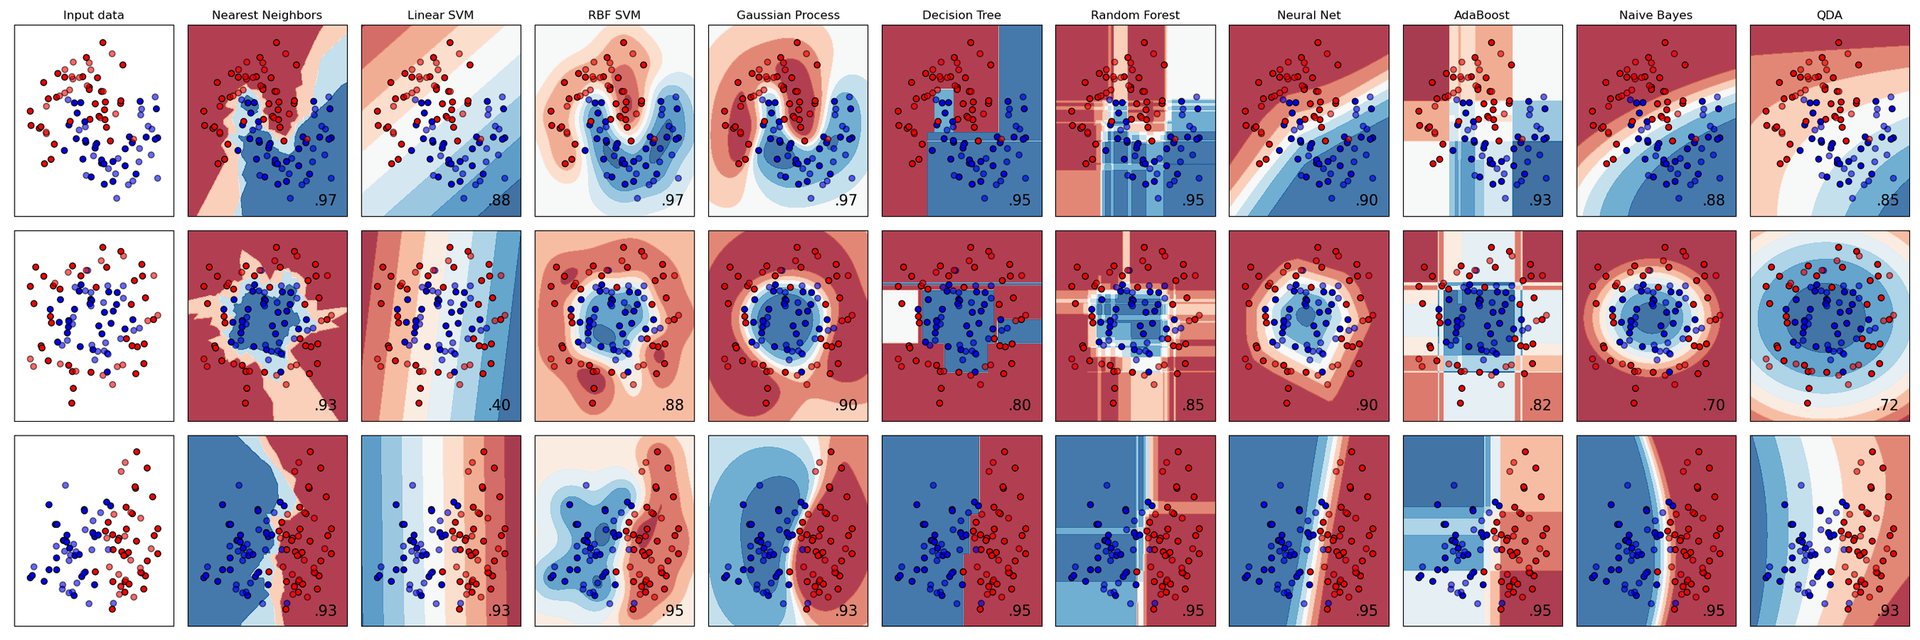
\includegraphics[width=5cm]{figures/img_p001_01.png}}

\begin{document}

% ============================================================ apertura parte 2
\titleframe
\addtocounter{framenumber}{1}

\begin{frame}{Contenido}
  \tableofcontents
\end{frame}

\begin{frame}{Dónde quedamos}
  \begin{columns}[T]
    \begin{column}{0.5\textwidth}
      \colhead{Parte 1}
      \small
      \begin{itemize}
        \item métricas, costos y threshold;
        \item workflow, EDA y baseline serio;
        \item validación cruzada estratificada, agrupada y temporal;
        \item ROC, PR y calibración;
        \item búsqueda de hiperparámetros: grid, random, halving y nested CV.
      \end{itemize}
    \end{column}
    \begin{column}{0.44\textwidth}
      \begin{keybox}[Pregunta puente]
        Ya sabemos evaluar y buscar configuraciones. ¿Qué modelos vale la pena optimizar, y cómo buscar mejor cuando cada entrenamiento es caro?
      \end{keybox}
    \end{column}
  \end{columns}
\end{frame}

\begin{frame}{El mapa de la sesión}
  \small
  \begin{enumerate}
    \item Árboles de decisión (CART), pruning y bias--variance.
    \item Ensembles: voting, bagging y boosting.
    \item Boosting moderno: XGBoost, LightGBM y CatBoost.
    \item Balanceo a nivel de datos y de modelo.
    \item CV para HPO y optimización bayesiana con Optuna.
    \item Hands-on y defensa técnica del primer experimento.
  \end{enumerate}
  \vspace{8pt}
  \begin{center}
    \Large\textbf{La historia completa es una cadena:} problema $\rightarrow$ datos $\rightarrow$ CV $\rightarrow$ métrica $\rightarrow$ threshold $\rightarrow$ decisión.
  \end{center}
\end{frame}

% ============================================================ p35
\section{CART: impurezas, splits y pruning}
\sectionframe{CART: impurezas, splits y pruning}

% ============================================================ p36
\begin{frame}{Por qué hablar de árboles en esta sesión}
  \begin{center}
    \large El árbol es el objeto más simple para entender\\[4pt]
    particiones, complejidad, sobreajuste, estabilidad y ensembles.
  \end{center}
  \begin{itemize}
    \item No buscamos hacer benchmarking de algoritmos.
    \item Buscamos entender por qué un modelo flexible puede ser frágil.
    \item El árbol es el \emph{learner} base de bagging y boosting.
  \end{itemize}
\end{frame}

% ============================================================ p37
\begin{frame}{¿Qué es un Decision Tree?}
  \large Un árbol de decisión es un modelo de \textbf{aprendizaje supervisado} que realiza predicciones mediante una \emph{estructura jerárquica de reglas de decisión}.
  \normalsize
  \begin{columns}[c]
    \begin{column}{0.47\textwidth}
      \colhead{Componentes principales:}
      \begin{itemize}
        \item \textbf{Nodo raíz}: primera decisión
        \item \textbf{Nodos internos}: reglas de división
        \item \textbf{Nodos hoja}: predicciones finales
        \item \textbf{Ramas}: caminos de decisión
      \end{itemize}
      \footnotesize\textbf{Ventajas}: interpretable, no requiere normalización, maneja features categóricas y numéricas.
    \end{column}
    \begin{column}{0.5\textwidth}
      \centering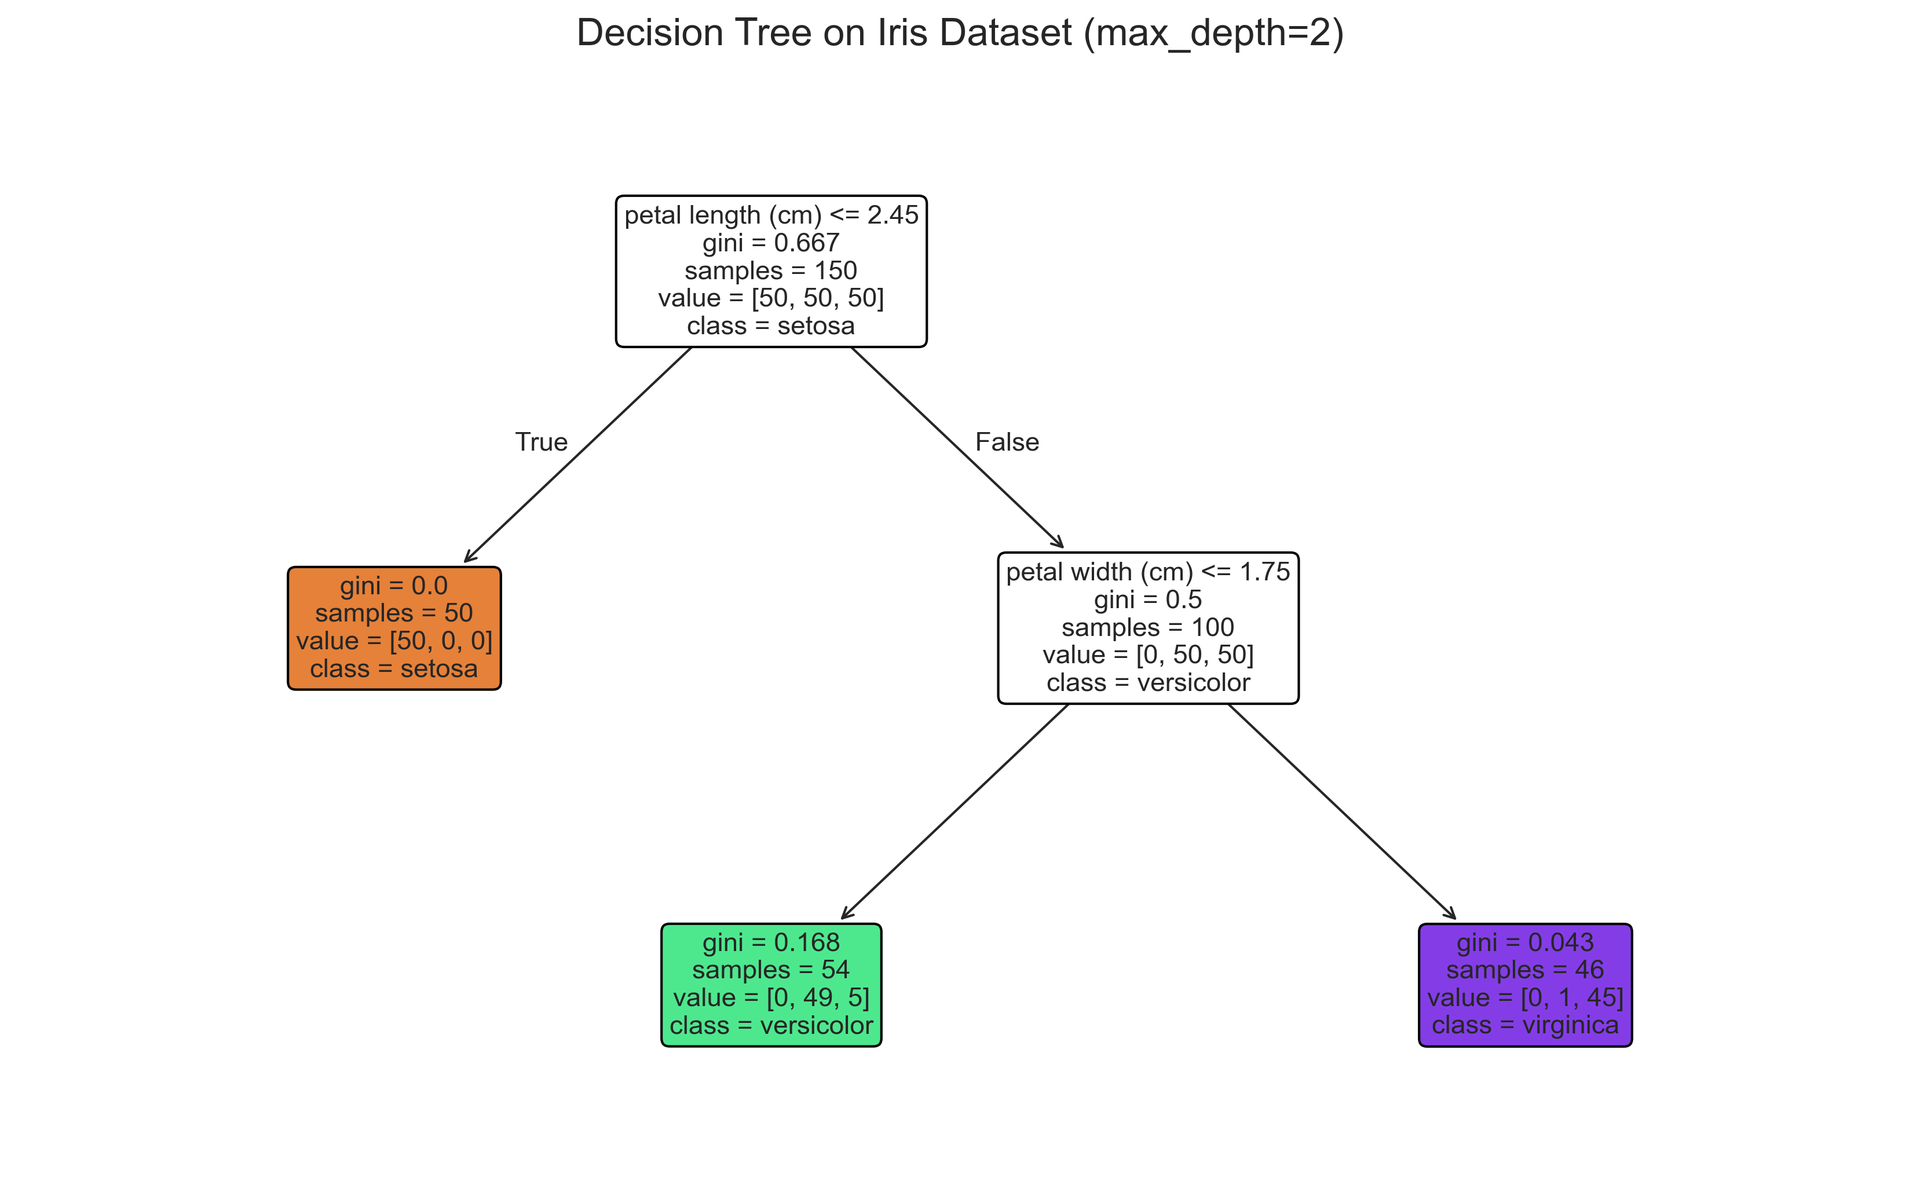
\includegraphics[width=\linewidth]{figures/img_p037_09.png}
    \end{column}
  \end{columns}
\end{frame}

% ============================================================ p40
\begin{frame}{Anatomía de un árbol de decisión}
  \centering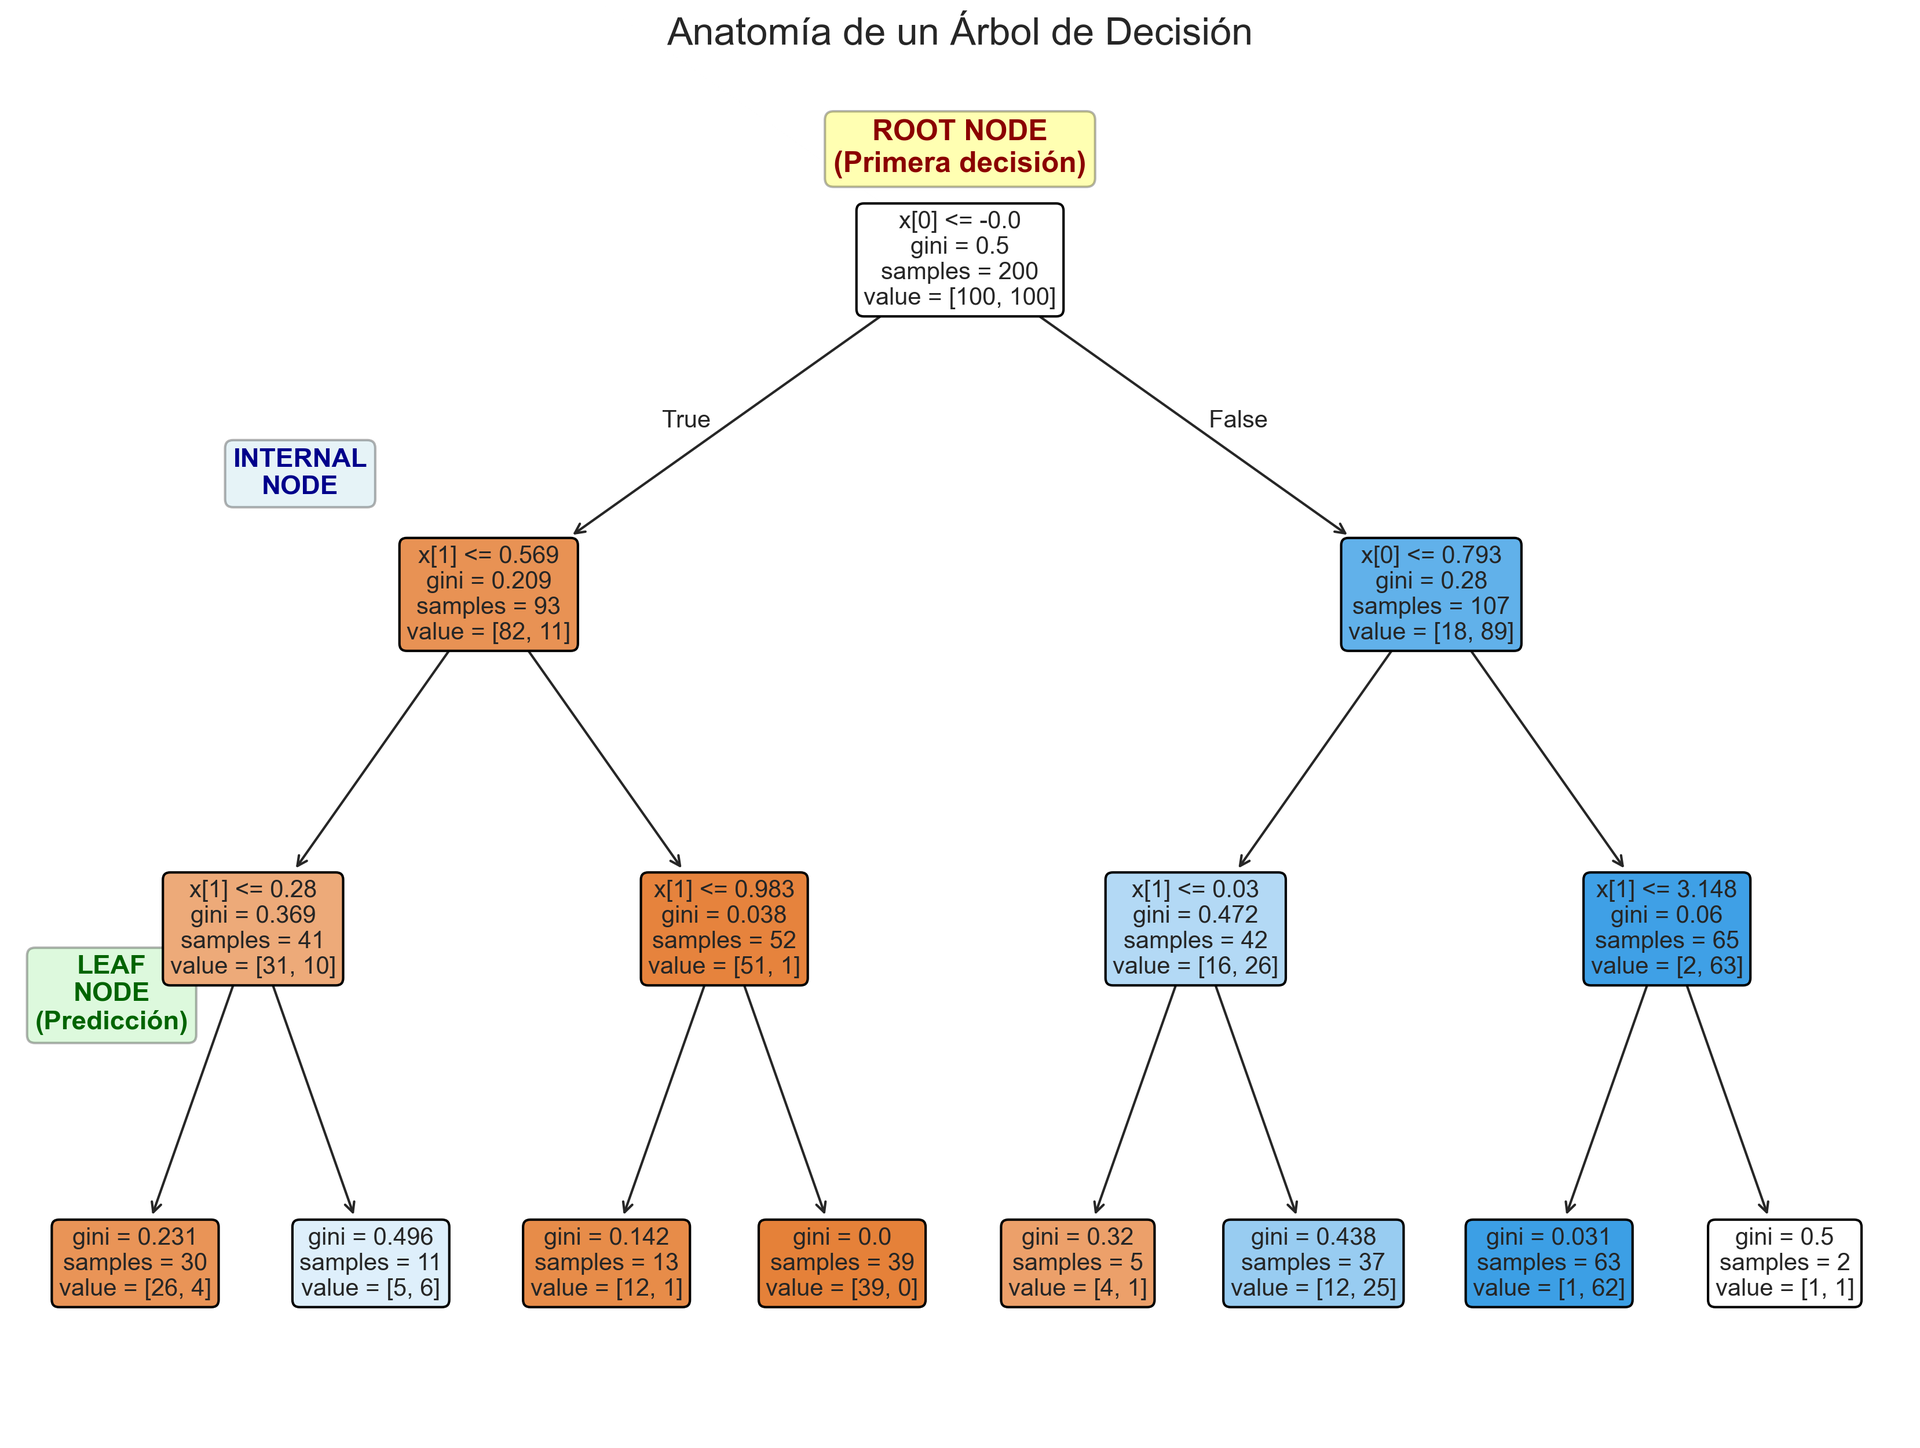
\includegraphics[height=0.38\textheight]{figures/img_p040_11.png}\par
  \raggedright
  \colhead{Proceso de predicción:}
  \small
  \begin{enumerate}\setlength{\itemsep}{0pt}
    \item Comenzar en el nodo raíz
    \item Evaluar condición del nodo actual
    \item Seguir rama correspondiente (True/False)
    \item Repetir hasta alcanzar un nodo hoja
    \item Retornar predicción del nodo hoja
  \end{enumerate}
\end{frame}

% ============================================================ p41 (+p42)
\begin{frame}{CART: Algoritmo fundamental}
  \textbf{CART} (\emph{Classification and Regression Trees}) construye árboles binarios mediante particiones recursivas que minimizan una función de costo.
  \relax{\large\[
    J(k, t_k) = \frac{m_{\text{left}}}{m} G_{\text{left}} + \frac{m_{\text{right}}}{m} G_{\text{right}}
  \]}
  \small
  \begin{itemize}
    \item $k$: feature seleccionado para el split; $t_k$: umbral para dividir;
    \item $G$: medida de impureza (Gini o Entropy);
    \item $m$: número total de muestras; $m_{\text{left}}$, $m_{\text{right}}$: muestras en cada hijo.
  \end{itemize}
\end{frame}

% ============================================================ p43
\begin{frame}{CART: Algoritmo paso a paso}
  \small
  \textbf{Procedimiento recursivo:}
  \begin{enumerate}
    \item \textbf{Inicio}: Conjunto completo de datos en raíz
    \item \textbf{Para cada nodo}:
    \begin{itemize}
      \item Evaluar todos los features
      \item Para cada feature, probar todos los \emph{thresholds} posibles
      \item Seleccionar $(k, t_k)$ que minimiza $J(k, t_k)$
      \item Crear dos nodos hijos con las particiones
    \end{itemize}
    \item \textbf{Recursión}: Repetir para cada hijo
    \item \textbf{Criterio de parada}:
    \begin{itemize}
      \item Profundidad máxima alcanzada
      \item Número mínimo de muestras no cumplido
      \item No hay reducción significativa de impureza
      \item Nodo puro (impureza $= 0$)
    \end{itemize}
  \end{enumerate}
\end{frame}

% ============================================================ p44
\begin{frame}{Propiedades de CART}
  \begin{columns}[T]
    \begin{column}{0.47\textwidth}
      \colhead{Ventajas:}
      \begin{itemize}
        \item Árboles binarios (fácil implementación)
        \item Maneja \emph{features} numéricos y categóricos
        \item Solución determinística
        \item No requiere normalización
        \item Robusto a \emph{outliers}
      \end{itemize}
      \vspace{4pt}
    \end{column}
    \begin{column}{0.47\textwidth}
      \vspace{6pt}
      \colhead{Desventajas:}
      \begin{itemize}
        \item \emph{Greedy algorithm} (no garantiza óptimo global)
        \item Sensible a rotaciones de datos
        \item Propenso a \emph{overfitting}
        \item Inestable (pequeños cambios $\rightarrow$ árbol diferente)
        \item Probabilidades mal calibradas (hojas puras $\rightarrow$ 0 o 1)
      \end{itemize}
    \end{column}
  \end{columns}
  \begin{rulebox}[Complejidad computacional]
    Entrenamiento: $O(n \cdot m \log_2(m))$ donde $n = $ features, $m = $ muestras
  \end{rulebox}
\end{frame}

% ============================================================ p46
\begin{frame}{Gini Impurity: Definición y derivación}
  \large La impureza de Gini mide la \textbf{probabilidad} de clasificar incorrectamente una muestra seleccionada aleatoriamente.\par
  \centering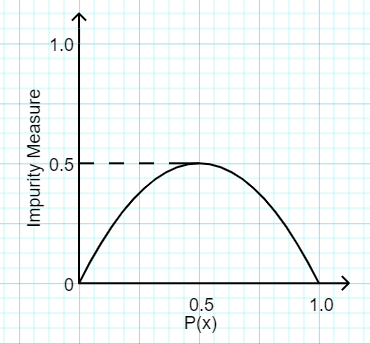
\includegraphics[height=0.5\textheight]{figures/img_p046_12.png}\par
  \footnotesize Máximo binario: Gini $0{,}5$, entropía $1{,}0$. Ambas miden qué tan mezclado está un nodo; los árboles buscan grupos más homogéneos.
\end{frame}

% ============================================================ p48
\begin{frame}{Gini Impurity: Definición y derivación}
  \large
  \textbf{Fórmula:}
  \[ G_i = 1 - \sum_{k=1}^{n} p_{i,k}^2 \]
  \textbf{Donde:}
  \begin{itemize}
    \item $p_{i,k}$: proporción de muestras de clase $k$ en el nodo $i$
    \item $n$: número total de clases
    \item Rango: $[0, 1 - \frac{1}{n}]$
    \item $G_i = 0$ indica pureza perfecta (todas las muestras de una clase)
  \end{itemize}
\end{frame}

% ============================================================ p49
\begin{frame}{Gini Impurity: Interpretación probabilística}
  \textbf{Derivación intuitiva:}\\
  Si seleccionamos dos muestras al azar del nodo $i$:
  \begin{itemize}
    \item Probabilidad de que la primera sea clase $k$: $p_{i,k}$
    \item Probabilidad de que la segunda NO sea clase $k$: $(1 - p_{i,k})$
    \item Probabilidad de clasificación incorrecta para clase $k$: $p_{i,k}(1 - p_{i,k})$
  \end{itemize}
  Sumando sobre todas las clases:
  \[
    G_i = \sum_{k=1}^{n} p_{i,k}(1 - p_{i,k}) = \sum_{k=1}^{n} p_{i,k} - \sum_{k=1}^{n} p_{i,k}^2 = 1 - \sum_{k=1}^{n} p_{i,k}^2
  \]
  \begin{goldbox}[Casos extremos]
    \textbf{Máxima impureza} (distribución uniforme): $G = 1 - \frac{1}{n}$\\
    \textbf{Mínima impureza} (nodo puro): $G = 0$
  \end{goldbox}
\end{frame}

% ============================================================ p50
\begin{frame}{Gini Impurity: Ejemplo numérico}
  \textbf{Escenario}: Nodo con 54 muestras
  \begin{itemize}
    \item Clase 0 (setosa): 0 muestras $\rightarrow p_{i,0} = 0/54 = 0$
    \item Clase 1 (versicolor): 49 muestras $\rightarrow p_{i,1} = 49/54 \approx 0{,}907$
    \item Clase 2 (virginica): 5 muestras $\rightarrow p_{i,2} = 5/54 \approx 0{,}093$
  \end{itemize}
  \textbf{Cálculo de Gini:}
  \begin{gather*}
    G_i = 1 - (0^2 + 0{,}907^2 + 0{,}093^2)\\
    G_i = 1 - (0 + 0{,}823 + 0{,}009) = 1 - 0{,}832 = 0{,}168
  \end{gather*}
  \begin{block}{Interpretación}
    \small $G = 0{,}168$ indica impureza moderada. El nodo está dominado por versicolor (90.7\,\%) pero tiene algunas virginicas (9.3\,\%).
  \end{block}
\end{frame}

% ============================================================ p52
\begin{frame}{Entropy: Definición desde la teoría de la información}
  \relax{\large\textbf{Entropía}: mide el grado de \emph{incertidumbre} o \emph{desorden} en un conjunto de datos.\par}
  \begin{itemize}
    \item Concepto introducido en 1948 por \emph{Claude Shannon} en su artículo \emph{A Mathematical Theory of Communication}.
    \item La entropía cuantifica la cantidad \emph{promedio de información necesaria} para describir una variable aleatoria.
    \item Cuanto mayor es la entropía, mayor es la incertidumbre; una buena división reduce esa entropía, creando nodos más puros.
  \end{itemize}
\end{frame}

% ============================================================ p54
\begin{frame}{Entropy: Definición desde teoría de información}
  \textbf{Fórmula:}
  \[ H_i = -\sum_{k=1}^{n} p_{i,k} \log_2(p_{i,k}) \]
  \textbf{Donde:}
  \begin{itemize}
    \item $p_{i,k}$: proporción de clase $k$ en nodo $i$
    \item $\log_2$: logaritmo base 2 (medida en bits)
    \item Convención: $0 \log_2(0) = 0$
    \item Rango: $[0, \log_2(n)]$
    \item $H_i = 0$ cuando hay una sola clase
  \end{itemize}
  \begin{rulebox}[Interpretación de Shannon]
    Número promedio de bits necesarios para codificar la información.
  \end{rulebox}
\end{frame}

% ============================================================ p56
\begin{frame}{Entropy: Ejemplo numérico y comparación}
  \textbf{Mismo escenario anterior}: 54 muestras (0 setosa, 49 versicolor, 5 virginica)
  \begin{gather*}
    H_i = -(0 \cdot \log_2(0) + 0{,}907 \cdot \log_2(0{,}907) + 0{,}093 \cdot \log_2(0{,}093))\\
    H_i = -(0 + 0{,}907 \cdot (-0{,}141) + 0{,}093 \cdot (-3{,}426))\\
    H_i = -(-0{,}128 - 0{,}319) = 0{,}447 \text{ bits}
  \end{gather*}
  \begin{columns}[c]
    \begin{column}{0.5\textwidth}
      \colhead{Comparación Gini vs Entropy:}
      \begin{itemize}
        \item Gini: $G = 0{,}168$
        \item Entropy: $H = 0{,}447$
      \end{itemize}
    \end{column}
    \begin{column}{0.42\textwidth}
      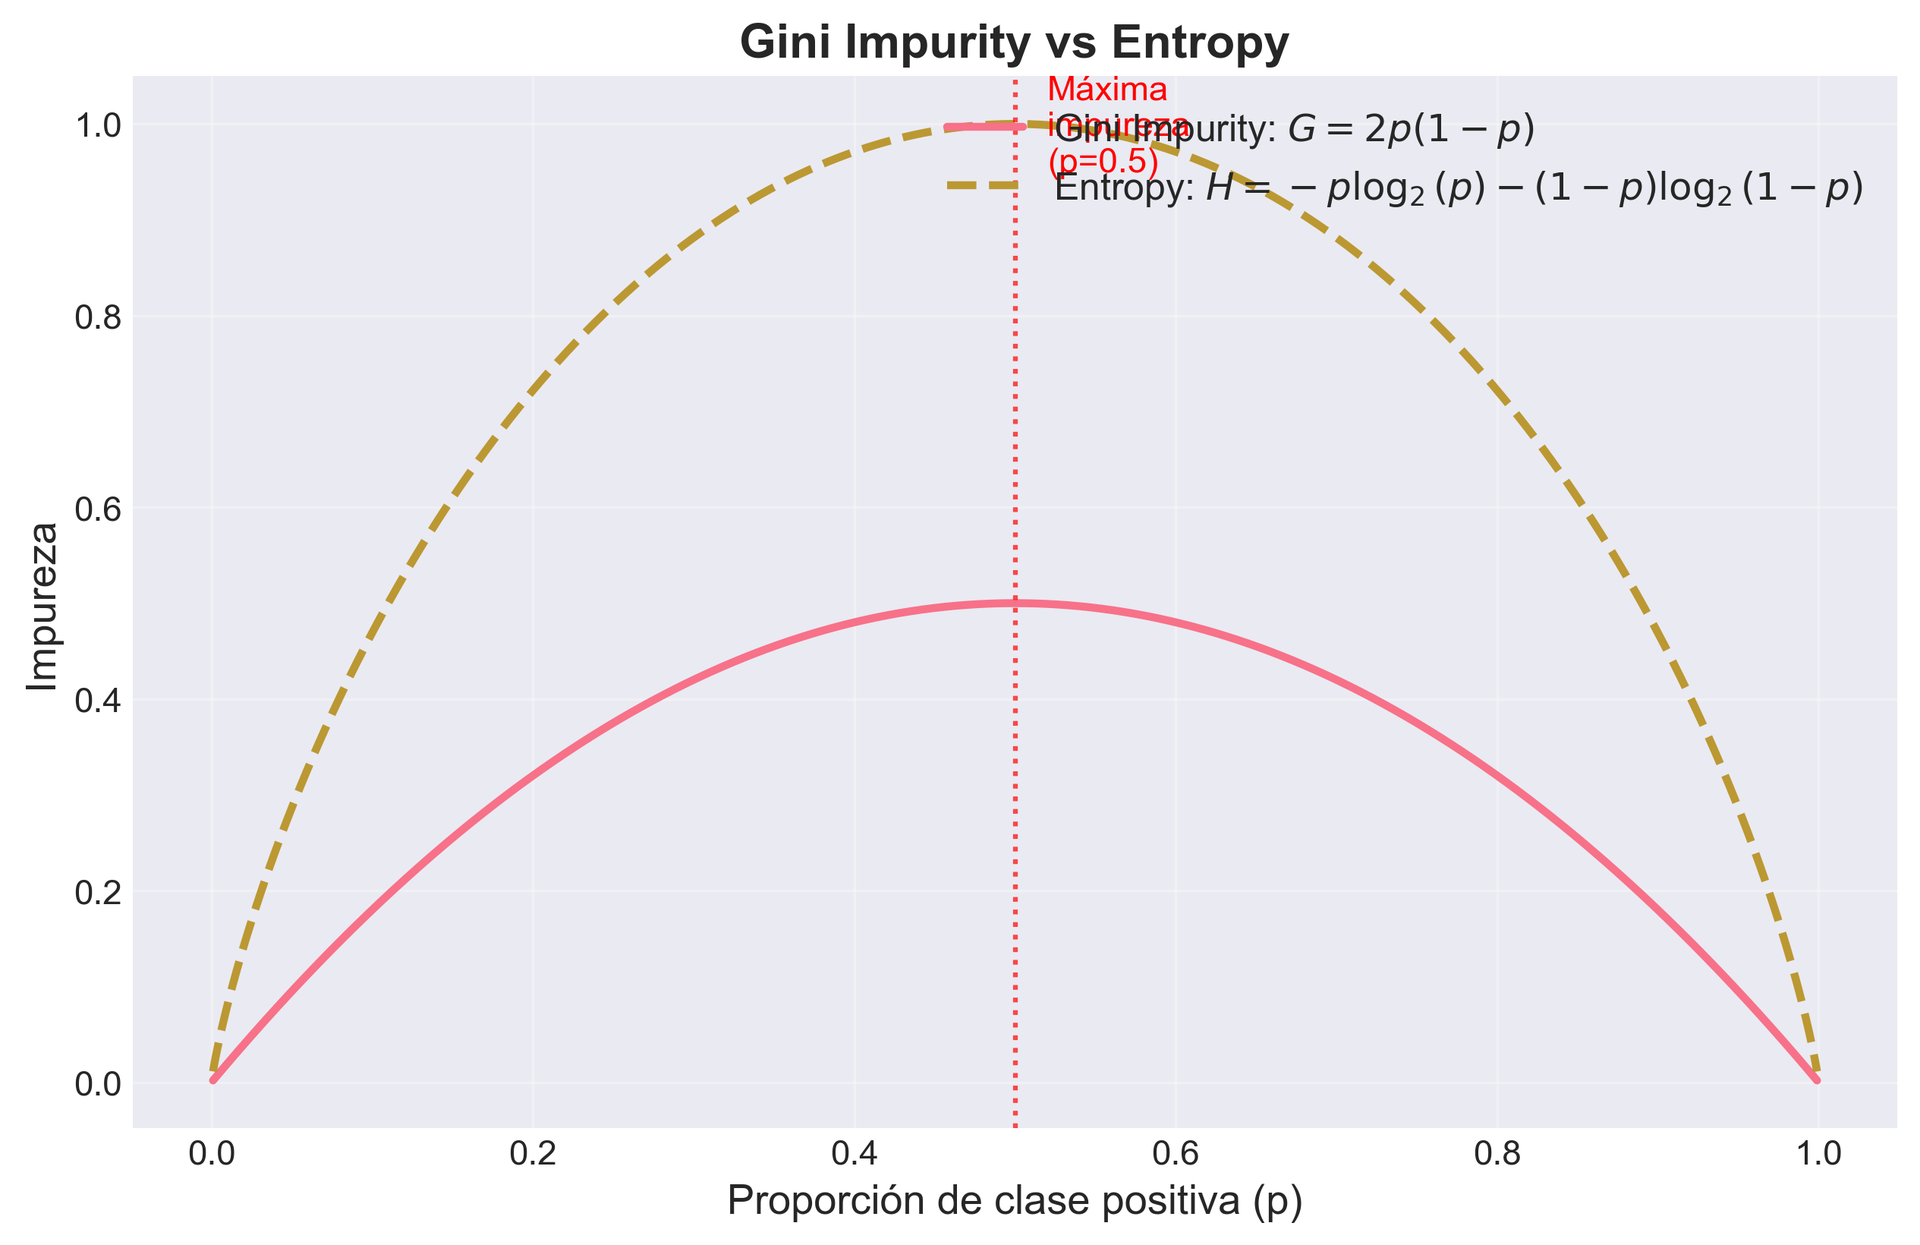
\includegraphics[width=0.9\linewidth]{figures/img_p056_15.png}
    \end{column}
  \end{columns}
\end{frame}

% ============================================================ p57 (+p58)
\begin{frame}{Information Gain: Reducción de entropía}
  El \textbf{Information Gain} mide cuánta incertidumbre se reduce al hacer un split.
  \relax{\large\[ IG = H_{\text{parent}} - \sum_{j \in \{\text{left, right}\}} \frac{n_j}{n} H_j \]}
  \small
  \begin{itemize}
    \item $H_{\text{parent}}$: entropía del nodo padre; $H_j$: entropía del hijo $j$;
    \item $n_j$: muestras en el hijo $j$; $n$: muestras totales.
  \end{itemize}
  \begin{goldbox}[Objetivo]
    Maximizar IG equivale a minimizar la entropía ponderada de los hijos.
  \end{goldbox}
\end{frame}

% ============================================================ p60
\begin{frame}{Gini vs Entropy: ¿Cuál usar?}
  \begin{columns}[T]
    \begin{column}{0.47\textwidth}
      \colhead{Gini Impurity:}
      \small
      \begin{itemize}
        \item Más rápido computacionalmente
        \item No requiere logaritmos
        \item Tiende a aislar clase más frecuente
        \item Default en \emph{scikit-learn}
        \item Rango: $[0, 0{,}5]$ (binario)
      \end{itemize}
    \end{column}
    \begin{column}{0.47\textwidth}
      \colhead{Entropy:}
      \small
      \begin{itemize}
        \item Computacionalmente más costoso
        \item Base teórica más sólida
        \item Tiende a árboles más balanceados
        \item Penaliza más fuertemente impureza
        \item Rango: $[0, 1]$ (binario)
      \end{itemize}
    \end{column}
  \end{columns}
  \begin{block}{Recomendación práctica}\footnotesize
    \textbf{En la mayoría de casos producen árboles similares}. Usar Gini por defecto (velocidad). Probar Entropy si se buscan árboles más balanceados. Con desbalance, ambas quedan dominadas por la clase mayoritaria: \texttt{class\_weight} modifica las proporciones $p_k$.
  \end{block}
\end{frame}

% ============================================================ p61
\subsection{Pruning}
\sectionframe{Pruning: controlar la\\complejidad del árbol}

% ============================================================ p62-63
\placedframe{figures/img_p062_17.png}{38}{20}{413}
\placedframe{figures/img_p063_18.png}{38}{20}{413}

% ============================================================ p68
\begin{frame}{El problema del overfitting}
  Sin restricciones, un árbol de decisión puede crecer hasta memorizar perfectamente el conjunto de entrenamiento.
  \begin{columns}[c]
    \begin{column}{0.47\textwidth}
      \colhead{Síntomas de overfitting:}
      \begin{itemize}
        \item Árbol muy profundo
        \item Hojas con pocas muestras
        \item Error training $\approx 0$
        \item Error test $\gg$ Error training
        \item Decisiones \emph{boundary} muy irregulares
      \end{itemize}
    \end{column}
    \begin{column}{0.5\textwidth}
      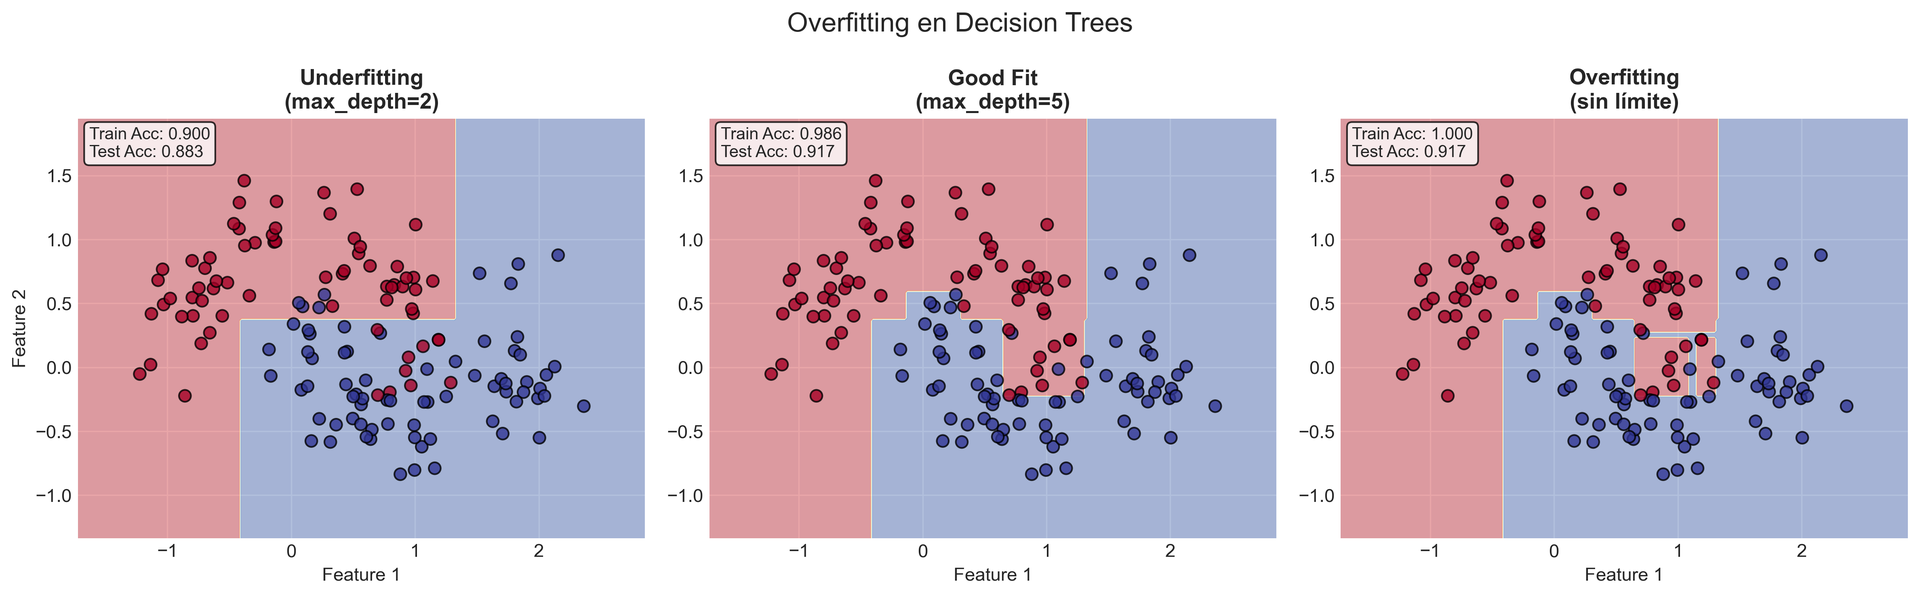
\includegraphics[width=\linewidth]{figures/img_p068_21.png}
    \end{column}
  \end{columns}
  \begin{rulebox}[Modelos no paramétricos]
    Decision trees son modelos no paramétricos: el número de parámetros crece con los datos
  \end{rulebox}
\end{frame}

% ============================================================ p69
\begin{frame}{Pre-pruning: hiperparámetros de regularización}
  \small
  \textbf{Pre-pruning}: Detener crecimiento durante construcción
  \begin{itemize}
    \item \texttt{max\_depth}: Profundidad máxima del árbol
    \begin{itemize}\scriptsize
      \item Típico: 3--10 para evitar overfitting
      \item $\infty$ permite memorización completa
    \end{itemize}
    \item \texttt{min\_samples\_split}: Mínimo de muestras para dividir nodo
    \begin{itemize}\scriptsize
      \item Típico: 2--20
      \item Valores altos $\rightarrow$ árboles más simples
    \end{itemize}
    \item \texttt{min\_samples\_leaf}: Mínimo de muestras en hoja
    \begin{itemize}\scriptsize
      \item Asegura generalización
      \item Evita hojas con muestras individuales
    \end{itemize}
    \item \texttt{max\_leaf\_nodes}: Número máximo de hojas
    \begin{itemize}\scriptsize
      \item Control directo de complejidad
      \item Alternativa a \texttt{max\_depth}
    \end{itemize}
  \end{itemize}
\end{frame}

% ============================================================ P2 (nuevo, post-pruning)
\begin{frame}[fragile]{Post-pruning por costo-complejidad}
  \begin{center}
    Se deja crecer el árbol y luego se podan las ramas que no justifican su complejidad.
  \end{center}
  \relax{\large\[ R_\alpha(T) = R(T) + \alpha\,|T| \]}
  \small
  \begin{itemize}
    \item $R(T)$: error (impureza total) del árbol; $|T|$: número de hojas;
    \item $\alpha$ grande $\rightarrow$ árbol más pequeño;
    \item \texttt{ccp\_alpha} se elige \textbf{con CV}, como cualquier hiperparámetro.
  \end{itemize}
\begin{lstlisting}[basicstyle=\ttfamily\scriptsize,columns=fullflexible,keepspaces=true]
path = DecisionTreeClassifier().cost_complexity_pruning_path(X_train, y_train)
grid = GridSearchCV(DecisionTreeClassifier(), {"ccp_alpha": path.ccp_alphas},
                    cv=skf, scoring="average_precision")
\end{lstlisting}
\end{frame}

% ============================================================ p70
\begin{frame}{Efecto de la regularización}
  \centering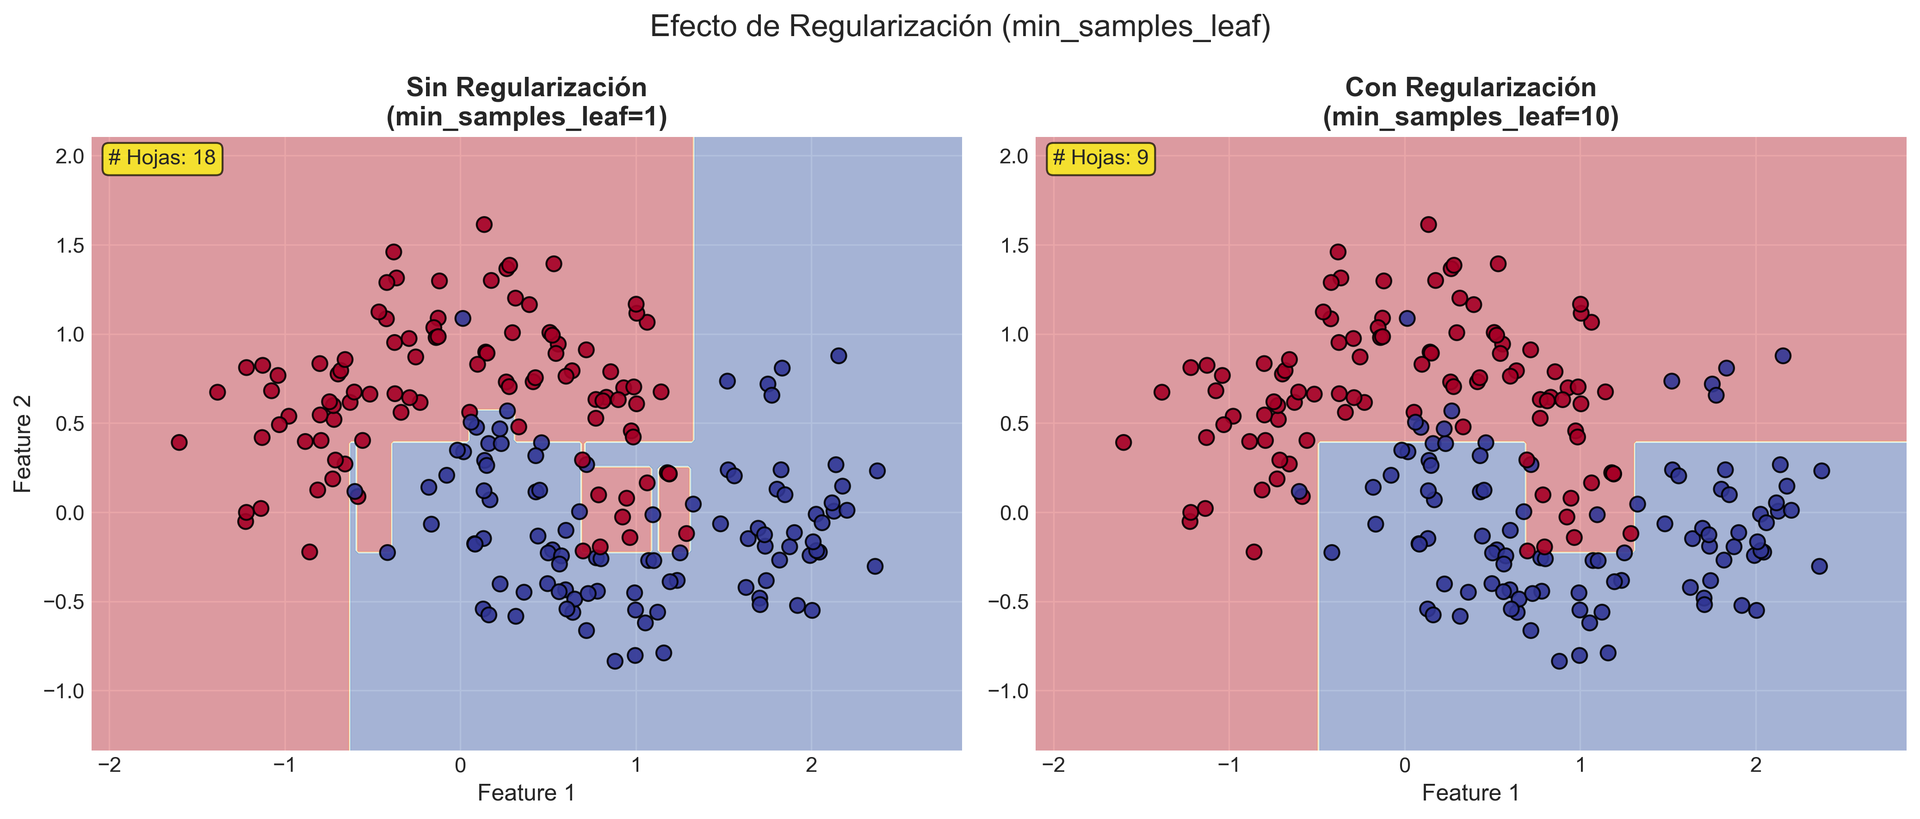
\includegraphics[width=0.92\textwidth]{figures/img_p070_22.png}\par
  \raggedright
  \textbf{Izquierda}: Sin regularización (\emph{overfitting})\\
  \textbf{Derecha}: Con \texttt{min\_samples\_leaf=4} (mejor generalización)
\end{frame}

% ============================================================ BV (nuevo separador)
\section{Bias--variance}
\sectionframe{Bias--variance: complejidad y error}

% ============================================================ p64
\begin{frame}{Profundidad: potencia y fragilidad}
  \large
  \begin{columns}[T]
    \begin{column}{0.45\textwidth}
      \colhead{Árbol poco profundo}
      \begin{itemize}
        \item reglas más simples;
        \item mayor estabilidad;
        \item posible underfitting;
        \item lectura más fácil.
      \end{itemize}
    \end{column}
    \begin{column}{0.45\textwidth}
      \colhead{Árbol muy profundo}
      \begin{itemize}
        \item reglas muy específicas;
        \item alta sensibilidad al dato;
        \item posible overfitting;
        \item peor generalización.
      \end{itemize}
    \end{column}
  \end{columns}
  \vspace{8pt}
  \begin{center}
    La profundidad aumenta capacidad, pero también puede aumentar fragilidad.
  \end{center}
\end{frame}

% ============================================================ p65
\begin{frame}{Bias--variance: dos formas de equivocarse}
  \centering
  \begin{tabular}{@{}l L{0.3\textwidth} L{0.3\textwidth}@{}}
    \toprule
    \hrow \textbf{Concepto} & Qué significa & Síntoma típico \\
    \midrule
    \textbf{Alto bias} & el modelo es demasiado rígido & falla incluso en train \\
    \textbf{Alta variance} & el modelo es demasiado sensible al dataset observado & funciona en train y falla fuera de muestra \\
    \bottomrule
  \end{tabular}
  \vspace{10pt}
  \raggedright\large
  \begin{itemize}
    \item Bias--variance no es un adorno teórico: es lenguaje para pensar complejidad, estabilidad y error.
  \end{itemize}
\end{frame}

% ============================================================ BV1 (nuevo)
\begin{frame}{Descomposición bias--variance}
  \small Con $y = f(x) + \varepsilon$ y esperanza sobre datasets de entrenamiento:
  \[ \mathbb{E}\big[(y - \hat{f}(x))^2\big] = \underbrace{\big(\mathbb{E}[\hat{f}(x)] - f(x)\big)^2}_{\text{Bias}^2} + \underbrace{\mathbb{E}\big[(\hat{f}(x) - \mathbb{E}[\hat{f}(x)])^2\big]}_{\text{Variance}} + \underbrace{\sigma^2}_{\text{ruido}} \]
  \centering
  \begin{tabular}{@{}l c c@{}}
    \toprule
    \hrow \textbf{Modelo} & Bias & Variance \\
    \midrule
    Árbol profundo & bajo & alta \\
    \emph{Stump} (profundidad 1) & alto & baja \\
    Árbol podado (\texttt{ccp\_alpha}) & compromiso & compromiso \\
    \bottomrule
  \end{tabular}
  \raggedright
  \begin{keybox}[Conexión con la CV]
    La variance se observa en la dispersión del score entre folds.
  \end{keybox}
\end{frame}

% ============================================================ BV2 (nuevo): ejemplo numérico
\begin{frame}{Descomposición bias--variance: ejemplo numérico}
  \small Sin ruido ($\sigma^2 = 0$). Verdad en $x$: $f(x) = 5$. Se entrena 3 veces con muestras distintas y los modelos predicen $4$, $6$ y $8$.
  \par\vspace{2pt}
  \centering
  \begin{tikzpicture}[x=1.05cm,y=0.8cm]
    \draw[-{Stealth[length=2mm]},mlgray] (2.6,0) -- (9.4,0);
    \foreach \v in {3,...,9} \draw[mlgray] (\v,0.07) -- (\v,-0.07) node[below=-1pt,font=\tiny,text=mlgray] {\v};
    \foreach \v in {4,6,8} \fill[eafitneon] (\v,0.3) circle (2.6pt);
    \node[right,font=\scriptsize,text=eafitneon] at (8.15,0.3) {predicciones};
    \draw[{Stealth[length=1.6mm]}-{Stealth[length=1.6mm]},eafitneon] (4,0.75) -- (8,0.75) node[midway,above=-1pt,font=\tiny] {dispersión alrededor de $m$: variance};
    \draw[mlred,very thick] (5,-0.35) -- (5,0.55);
    \draw[mlteal,very thick,dashed] (6,-0.35) -- (6,0.2);
    \draw[{Stealth[length=1.6mm]}-{Stealth[length=1.6mm]},mlred] (5,-0.6) -- (6,-0.6) node[midway,below=-1pt,font=\tiny] {bias $=1$};
    \node[left,font=\scriptsize,text=mlred] at (4.95,-0.6) {verdad $f=5$};
    \node[right,font=\scriptsize,text=mlteal] at (6.05,-0.6) {promedio $m=6$};
  \end{tikzpicture}
  \par\vspace{2pt}
  \footnotesize
  \begin{tabular}{@{}l l r@{}}
    \toprule
    \hrow \textbf{Término} & Cálculo & Valor \\
    \midrule
    \textbf{Error total} & $\big[(5-4)^2 + (5-6)^2 + (5-8)^2\big]/3 = (1+1+9)/3$ & $3{,}67$ \\
    \textbf{Bias$^2$} & $(m - f)^2 = (6-5)^2$ & $1$ \\
    \textbf{Variance} & $\big[(4-6)^2 + (6-6)^2 + (8-6)^2\big]/3 = (4+0+4)/3$ & $2{,}67$ \\
    \midrule
    \textbf{Bias$^2$ + Variance} & $1 + 2{,}67$ & $\mathbf{3{,}67}$ \\
    \bottomrule
  \end{tabular}
  \par\vspace{3pt}
  \raggedright\footnotesize El error se parte exacto: lejanía del promedio a la verdad (bias$^2$) + dispersión de los modelos (variance).
\end{frame}

% ============================================================ p66-67
\placedframe{figures/img_p066_19.png}{38}{20}{413}
\placedframe{figures/img_p067_20.png}{38}{20}{413}

% ============================================================ p71
\section{Ensembles como remedios arquitectónicos}
\sectionframe{Ensembles: remedios arquitectónicos\\para bias y variance}

% ============================================================ p72
\begin{frame}{¿Qué es Ensemble Learning?}
  \relax{\large\textbf{Principio fundamental}: Combinar múltiples modelos (\emph{weak learners}) para crear un predictor más robusto y preciso.\par}
  \begin{columns}[c]
    \begin{column}{0.47\textwidth}
      \textbf{Analogía}:
      \begin{itemize}
        \item Pregunta compleja a 1000 personas
        \item Promedia sus respuestas
        \item Resultado mejor que respuesta de experto
      \end{itemize}
      \textbf{Wisdom of the Crowd}
    \end{column}
    \begin{column}{0.5\textwidth}
      \centering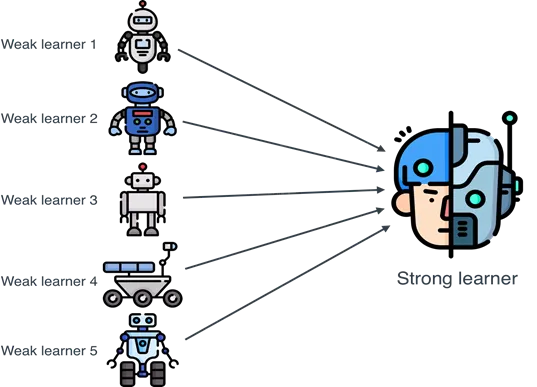
\includegraphics[width=\linewidth]{figures/img_p072_23.png}
    \end{column}
  \end{columns}
\end{frame}

% ============================================================ p73
\begin{frame}{¿Qué es Ensemble Learning?}
  \vfill
  \Large
  \textbf{Fórmula general}:
  \[ \hat{y}_{\text{ensemble}} = f(\hat{y}_1, \hat{y}_2, \ldots, \hat{y}_M) \]
  Donde $f$ es agregación (promedio, votación, ponderado)
  \vfill
\end{frame}

% ============================================================ p74
\imageframe{figures/img_p074_24.png}

% ============================================================ p75
\begin{frame}{¿Por qué funciona Ensemble Learning?}
  \textbf{Requisito clave}: Los modelos deben ser DIVERSOS (errores no correlacionados)\\
  \textbf{Matemática básica}:\\
  Para $M$ modelos independientes con error $\epsilon$ cada uno:
  \[ \text{Error}_{\text{ensemble}} \approx \frac{\epsilon}{\sqrt{M}} \quad\text{(idealización)} \]
  Con correlación $\rho$ entre modelos: $\;\mathrm{Var} = \rho\,\sigma^2 + \frac{1 - \rho}{M}\,\sigma^2$: la diversidad importa.
  \begin{rulebox}[Ley de los grandes números]
    Con suficientes \emph{weak learners} independientes, el \emph{ensemble} converge a la predicción correcta
  \end{rulebox}
\end{frame}

% ============================================================ p76-78
\imageframe{figures/img_p077_26.jpg}
\imageframe{figures/img_p078_27.png}

% ============================================================ p79
\subsection{Voting Classifiers}
\sectionframe{Votación: El Ensemble Más Simple}

% ============================================================ p80
\begin{frame}{Voting Classifiers: Concepto}
  \begin{columns}[c]
    \begin{column}{0.55\textwidth}
      {\Large Combina predicciones de múltiples modelos diferentes mediante votación.\par}
      \vspace{12pt}
      \begin{block}{Idea central}
        \small Entrenar varios clasificadores distintos (SVM, Logistic Regression, Decision Tree, etc.) y agregar sus predicciones.
      \end{block}
    \end{column}
    \begin{column}{0.4\textwidth}
      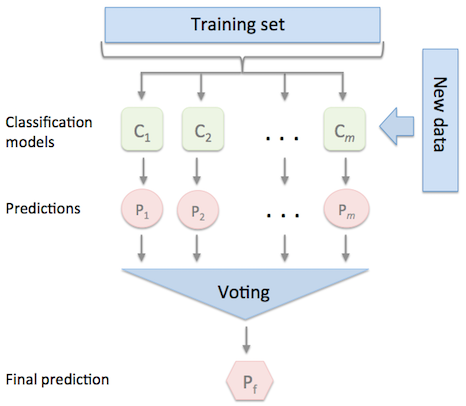
\includegraphics[width=\linewidth]{figures/img_p080_28.png}
    \end{column}
  \end{columns}
\end{frame}

% ============================================================ p81
\begin{frame}{Voting Classifiers: Concepto}
  \large
  \textbf{Hard Voting} (clasificación):
  \[ \hat{y} = \text{mode}(\hat{y}_1, \hat{y}_2, \ldots, \hat{y}_M) \]
  \textbf{Soft Voting} (probabilidades):
  \[ \hat{y} = \arg\max_k \sum_{m=1}^{M} p_m(y = k | x) \]
  \textbf{Regresión} (promedio):
  \[ \hat{y} = \frac{1}{M} \sum_{m=1}^{M} \hat{y}_m \]
\end{frame}

% ============================================================ p82
\begin{frame}{Hard vs Soft Voting}
  \small
  \setbeamerfont{itemize/enumerate body}{size=\small}
  \let\olditemize\itemize
  \renewcommand{\itemize}{\olditemize\setlength{\itemsep}{0pt}}
  \begin{columns}[T]
    \begin{column}{0.47\textwidth}
      \textbf{Hard Voting}:
      \begin{itemize}
        \item Cada modelo vota por una clase
        \item Gana la clase con más votos
        \item Simple pero puede perder información
      \end{itemize}
      \textbf{Ejemplo}:
      \begin{itemize}
        \item SVM: clase 1
        \item LR: clase 1
        \item DT: clase 0
        \item RF: clase 1
      \end{itemize}
      \textbf{Resultado}: clase 1 (3 votos vs 1)
    \end{column}
    \begin{column}{0.47\textwidth}
      \textbf{Soft Voting}:
      \begin{itemize}
        \item Promedia probabilidades
        \item Gana clase con mayor probabilidad promedio
        \item Usa confianza de cada modelo
      \end{itemize}
      \textbf{Ejemplo}:
      \begin{itemize}
        \item SVM: P(1)=0.6
        \item LR: P(1)=0.55
        \item DT: P(1)=0.45
        \item RF: P(1)=0.7
      \end{itemize}
      \textbf{Resultado}: P(1)=0.575 $\rightarrow$ clase 1
    \end{column}
  \end{columns}
  \begin{rulebox}[Requisito para Soft Voting]
    Todos los clasificadores deben tener método \texttt{predict\_proba()}
  \end{rulebox}
\end{frame}

% ============================================================ p83
\begin{frame}[t]{Requisito crítico: Diversidad}
  \vspace{-10pt}
  \textbf{Problema}: Si los clasificadores cometen los mismos errores, voting no ayuda.\\
  \textbf{Estrategias para diversidad}:
  \begin{itemize}\setlength{\itemsep}{0pt}
    \item Usar algoritmos muy diferentes (SVM, trees, logistic regression, etc.)
    \item Entrenar en diferentes subconjuntos de features
    \item Usar diferentes hiperparámetros
    \item Entrenar en diferentes subconjuntos de datos
  \end{itemize}
  % figure is cropped by the bottom of the slide in the original (bbox 60,119,393,407)
  \begin{tikzpicture}[remember picture,overlay]
    \begin{scope}
      \clip ([xshift=60pt,yshift=-119pt]current page.north west) rectangle ([xshift=393pt,yshift=-245pt]current page.north west);
      \node[anchor=north west,inner sep=0pt] at ([xshift=60pt,yshift=-119pt]current page.north west)
        {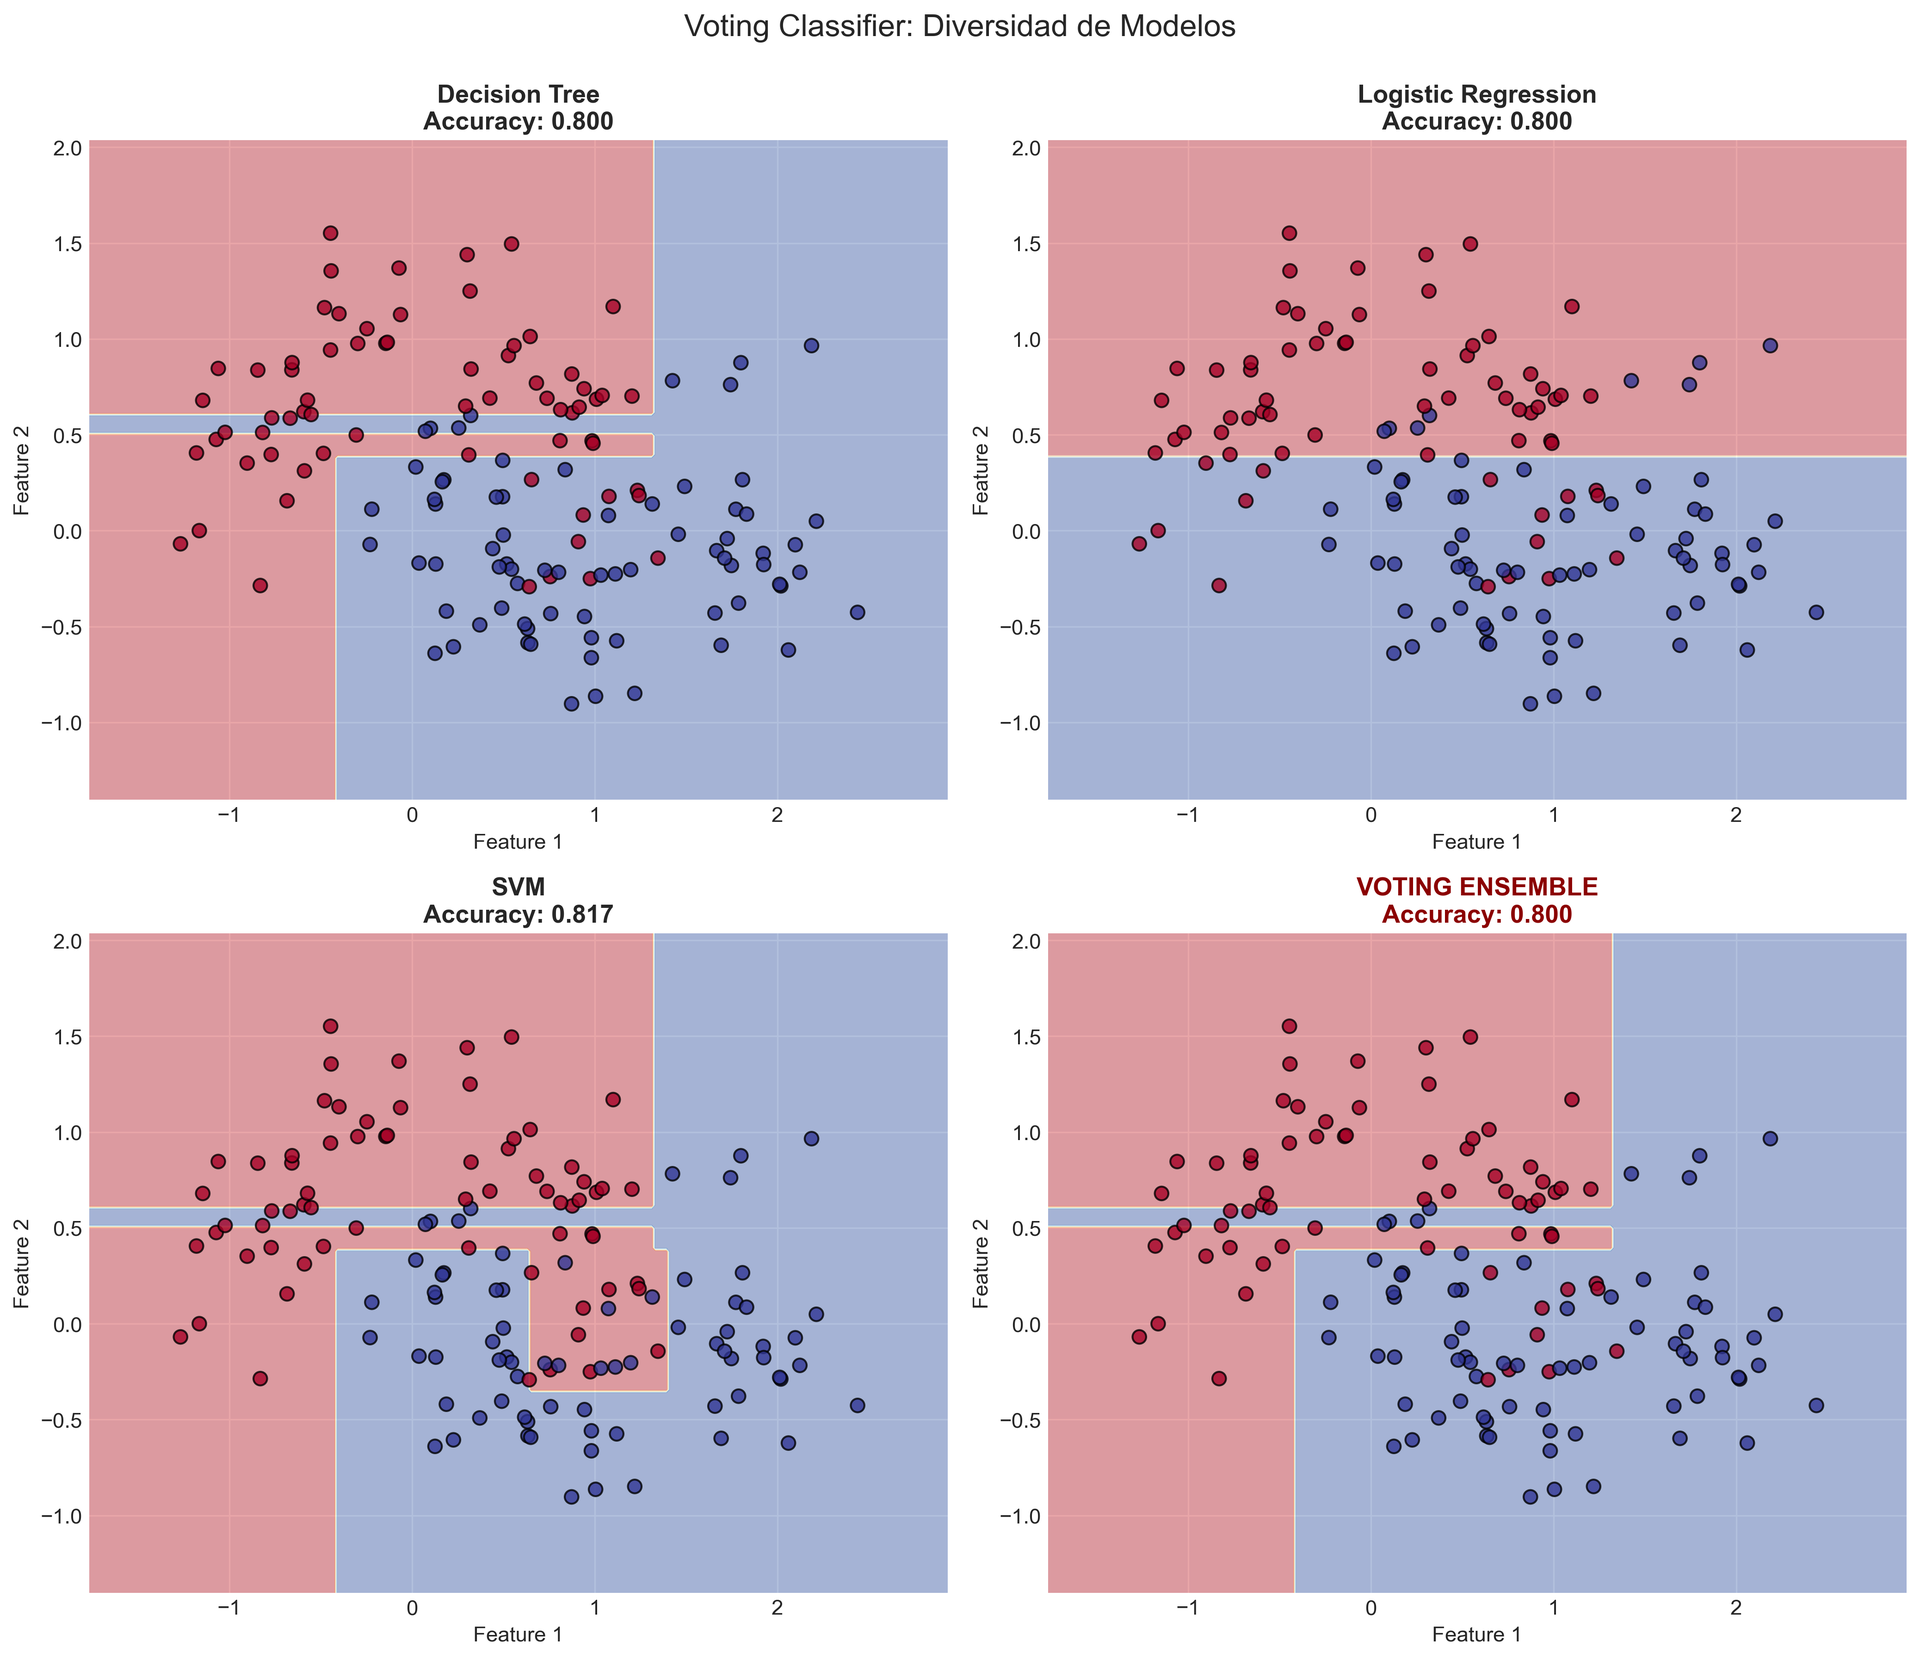
\includegraphics[width=333pt]{figures/img_p083_29.png}};
    \end{scope}
  \end{tikzpicture}
\end{frame}

% ============================================================ p84
\begin{frame}{Bagging: estabilizar modelos inestables}
  \begin{center}
    \large Si muchos árboles son sensibles al dato, agregarlos reduce la inestabilidad.
  \end{center}
  \begin{itemize}
    \item Se entrenan varios modelos sobre muestras bootstrap del dataset y se promedian.
    \item \textbf{Bagging ataca la variance}: promedia árboles profundos de bajo bias.
    \item \textbf{Random Forest} = bagging + submuestreo aleatorio de features en cada split.
    \item \texttt{BalancedRandomForestClassifier} (imblearn) combina bagging y balanceo.
  \end{itemize}
\end{frame}

% ============================================================ p85
\begin{frame}{Boosting: corregir errores de forma secuencial}
  \begin{center}
    \textbf{Boosting} construye una secuencia donde cada etapa intenta corregir los errores anteriores.
  \end{center}
  \centering\small
  \begin{tabular}{@{}l L{0.3\textwidth} L{0.3\textwidth}@{}}
    \toprule
    \hrow & Bagging & Boosting \\
    \midrule
    \textbf{Learner base} & profundo, bajo bias & débil, alto bias \\
    \textbf{Entrenamiento} & en paralelo & secuencial \\
    \textbf{Reduce} & variance & bias \\
    \textbf{Riesgo} & poco beneficio si los árboles están correlacionados & sobreajuste con demasiadas etapas \\
    \bottomrule
  \end{tabular}
  \raggedright
  \begin{rulebox}[Frontera]
    \small XGBoost, LightGBM y CatBoost se desarrollan en la sección siguiente; su búsqueda de hiperparámetros con Optuna, al final de hoy.
  \end{rulebox}
\end{frame}

% ============================================================ X1 (nuevo, opcional)
\begin{frame}[fragile]{(Opcional) Multiclase sin deep learning}
  \begin{columns}[T]
    \begin{column}{0.47\textwidth}
      \colhead{Modelos multiclase nativos}
      \small Árboles, Random Forest y gradient boosting predicen $K$ clases directamente.
      \vspace{6pt}

      \colhead{Reducción a problemas binarios}
      \begin{itemize}
        \item \textbf{One-vs-Rest}: $K$ clasificadores ``clase $k$ vs.\ resto''; gana el de mayor score.
        \item \textbf{One-vs-One}: $K(K-1)/2$ clasificadores por pares; gana la clase más votada.
      \end{itemize}
    \end{column}
    \begin{column}{0.47\textwidth}
\begin{lstlisting}[basicstyle=\ttfamily\scriptsize,columns=fullflexible,keepspaces=true]
from sklearn.multiclass import (
    OneVsRestClassifier, OneVsOneClassifier)
ovr = OneVsRestClassifier(
    DecisionTreeClassifier(max_depth=4))
\end{lstlisting}
      \begin{rulebox}[Cuidado]
        \small Codificar clases como números y usar un regresor impone un orden que no existe. Evaluar con macro-F1.
      \end{rulebox}
    \end{column}
  \end{columns}
\end{frame}

% ============================================================ GB0 (nuevo)
\section{Gradient boosting moderno}
\sectionframe{Gradient boosting moderno:\\XGBoost, LightGBM y CatBoost}

% ============================================================ GB1
\begin{frame}{Gradient boosting: sumar árboles que corrigen errores}
  \begin{center}
    Cada árbol nuevo $h_m$ se ajusta a lo que el modelo actual todavía hace mal:
    \[ F_m(x) = F_{m-1}(x) + \eta\, h_m(x) \]
  \end{center}
  \begin{columns}[T]
    \begin{column}{0.5\textwidth}
      \small
      \begin{itemize}
        \item $h_m$ aprende el \textbf{gradiente negativo} de la pérdida: en regresión, el residuo $y - F_{m-1}(x)$; en log-loss, $y - \hat{p}$;
        \item cada árbol es pequeño (alto bias): boosting \textbf{reduce bias} etapa a etapa;
        \item $\eta$ (\emph{learning rate}) encoge cada paso.
      \end{itemize}
    \end{column}
    \begin{column}{0.46\textwidth}
      \begin{keybox}[Regla práctica]
        \small $\eta$ pequeño + más árboles generaliza mejor, pero cuesta más. El número de árboles se elige con \textbf{early stopping}, no a mano.
      \end{keybox}
    \end{column}
  \end{columns}
\end{frame}

% ============================================================ GB2
\begin{frame}{XGBoost, LightGBM y CatBoost}
  \centering\scriptsize
  \begin{tabularx}{\textwidth}{@{}l >{\raggedright\arraybackslash}X >{\raggedright\arraybackslash}X >{\raggedright\arraybackslash}X@{}}
    \toprule
    \hrow & \textbf{XGBoost} & \textbf{LightGBM} & \textbf{CatBoost} \\
    \midrule
    \textbf{Idea clave} & objetivo regularizado ($\lambda$, $\gamma$) y aproximación de segundo orden & histogramas + crecimiento por hojas; muestreo GOSS & \emph{ordered boosting} contra el sesgo del target \\
    \textbf{Crecimiento} & por niveles (\texttt{max\_depth}) & por hojas (\texttt{num\_leaves}) & árboles simétricos (\texttt{depth}) \\
    \textbf{Categóricas} & requiere encoding (soporte nativo reciente) & nativas por partición óptima & nativas con \emph{ordered target statistics} \\
    \textbf{Fortaleza} & robusto, muy usado, buen manejo de faltantes & muy rápido en datos grandes & buenos defaults; muchas categóricas \\
    \textbf{Cuidado} & muchos hiperparámetros & sobreajusta con pocos datos & entrenamiento más lento en CPU \\
    \bottomrule
  \end{tabularx}
  \vspace{4pt}
  \raggedright\footnotesize Los tres implementan la misma idea; cambian cómo construyen cada árbol y cómo tratan categóricas. La teoría de cada uno se desarrolla en la sesión 2.
\end{frame}

% ============================================================ GB3
\begin{frame}{Crecimiento por niveles frente a por hojas}
  \begin{columns}[T]
    \begin{column}{0.5\textwidth}
      \centering
      \begin{tikzpicture}[level distance=0.72cm,
          every node/.style={circle,fill=eafitneon,inner sep=1.6pt},
          level 1/.style={sibling distance=1.5cm},level 2/.style={sibling distance=0.75cm}]
        \node {} child {node {} child {node {}} child {node {}}}
                 child {node {} child {node {}} child {node {}}};
      \end{tikzpicture}
      \par\footnotesize\textbf{Por niveles} (XGBoost): divide todas las hojas de un nivel antes de bajar.
      \par\vspace{6pt}
      \begin{tikzpicture}[level distance=0.62cm,
          every node/.style={circle,fill=mlred,inner sep=1.6pt},
          level 1/.style={sibling distance=1.5cm},level 2/.style={sibling distance=0.8cm},
          level 3/.style={sibling distance=0.6cm}]
        \node {} child {node {}}
                 child {node {} child {node {}} child {node {} child {node {}} child {node {}}}};
      \end{tikzpicture}
      \par\footnotesize\textbf{Por hojas} (LightGBM): divide la hoja que más reduce la pérdida.
    \end{column}
    \begin{column}{0.46\textwidth}
      \footnotesize
      \begin{itemize}
        \item por niveles: árboles balanceados; se controla con \texttt{max\_depth};
        \item por hojas: con el mismo número de hojas suele reducir más la pérdida, pero crea ramas profundas que sobreajustan con pocos datos;
        \item se controla con \texttt{num\_leaves} y \texttt{min\_child\_samples};
        \item CatBoost: árboles simétricos, mismo split en todo un nivel.
      \end{itemize}
      \begin{rulebox}[Regla]
        \footnotesize \texttt{num\_leaves} $< 2^{\texttt{max\_depth}}$ para no anular el límite de profundidad.
      \end{rulebox}
    \end{column}
  \end{columns}
\end{frame}

% ============================================================ GB4
\begin{frame}{Regularización y submuestreo}
  \centering\tiny\setlength{\tabcolsep}{3pt}
  \begin{tabularx}{\textwidth}{@{}l l l l >{\raggedright\arraybackslash}X@{}}
    \toprule
    \hrow \textbf{Palanca} & \textbf{XGBoost} & \textbf{LightGBM} & \textbf{CatBoost} & \textbf{Efecto} \\
    \midrule
    Tasa de aprendizaje & \texttt{learning\_rate} & \texttt{learning\_rate} & \texttt{learning\_rate} & pasos más pequeños, más árboles \\
    Número de árboles & \texttt{n\_estimators} & \texttt{n\_estimators} & \texttt{iterations} & fijar alto y cortar con early stopping \\
    Complejidad del árbol & \texttt{max\_depth} & \texttt{num\_leaves} & \texttt{depth} & menos capacidad, menos variance \\
    Mínimo por hoja & \texttt{min\_child\_weight} & \texttt{min\_child\_samples} & \texttt{min\_data\_in\_leaf} & evita hojas con muy pocos casos \\
    Penalización L1 / L2 & \texttt{reg\_alpha}, \texttt{reg\_lambda} & \texttt{reg\_alpha}, \texttt{reg\_lambda} & \texttt{l2\_leaf\_reg} & encoge los valores de las hojas \\
    Submuestreo de filas & \texttt{subsample} & \texttt{subsample}$^{*}$ & \texttt{subsample} & cada árbol ve otra muestra \\
    Submuestreo de columnas & \texttt{colsample\_bytree} & \texttt{colsample\_bytree} & \texttt{rsm} & árboles menos correlacionados \\
    Desbalance & \texttt{scale\_pos\_weight} & \texttt{scale\_pos\_weight} & \texttt{auto\_class\_weights} & pondera la clase rara \\
    \bottomrule
  \end{tabularx}
  \vspace{4pt}
  \raggedright\footnotesize El submuestreo trae a boosting una idea de bagging: introduce diversidad y reduce variance. Nombres según la API de scikit-learn de cada librería. $^{*}$En LightGBM requiere \texttt{subsample\_freq} $> 0$.
\end{frame}

% ============================================================ B0 (nuevo separador + p112-114)
\section{Balanceo: nivel de datos y de modelo}
\sectionframe{Balanceo: nivel de datos y de modelo}

\begin{frame}{El problema del desbalance de clases}
  \begin{columns}[T]
    \begin{column}{0.47\textwidth}
      \colhead{¿Cuándo ocurre?}
      \begin{itemize}
        \item fraude: $\approx 0{,}1$--$0{,}2$\,\% positivos;
        \item diagnóstico de enfermedades raras;
        \item churn: $\approx 5$\,\% abandona;
        \item detección de anomalías;
        \item multiclase: en \emph{Amazon reviews} domina 5 estrellas.
      \end{itemize}
    \end{column}
    \begin{column}{0.47\textwidth}
      \colhead{¿Por qué es problemático?}
      \begin{itemize}
        \item el modelo trivial obtiene alta accuracy;
        \item los algoritmos se sesgan hacia la mayoría;
        \item la clase rara queda ignorada.
      \end{itemize}
    \end{column}
  \end{columns}
  \vspace{6pt}
  \begin{keybox}[Recordatorio]
    99,8\,\% de aciertos y recall de fraude igual a cero: ya sabemos medirlo. Ahora, ¿cómo lo mejoramos?
  \end{keybox}
\end{frame}

% ============================================================ p115-118
\imageframe{figures/img_p115_37.png}
\imageframe{figures/img_p116_38.png}
\imageframe{figures/img_p117_39.png}
\imageframe{figures/img_p118_40.jpg}

% ============================================================ p119
\begin{frame}{Estrategias para datos desbalanceados}
  \textbf{Nivel de datos}:
  \begin{itemize}
    \item Ajustes \textbf{sólo} en \emph{train}; dev/test conservan distribución.
    \item \textbf{Undersampling}: Submuestreo (reducción) de la clase mayoritaria.
    \item \textbf{Oversampling}: Remuestreo (aumento) de clases minoritarias.
    \item Generación sintética
    \begin{itemize}
      \item \textbf{SMOTE}: Synthetic Minority Oversampling
      \item \textbf{Borderline-SMOTE}: sintéticos solo cerca de la frontera de decisión
      \item \textbf{ADASYN}: Adaptive Synthetic Sampling
    \end{itemize}
  \end{itemize}
\end{frame}

% ============================================================ p120
\begin{frame}{Estrategias para datos desbalanceados}
  \centering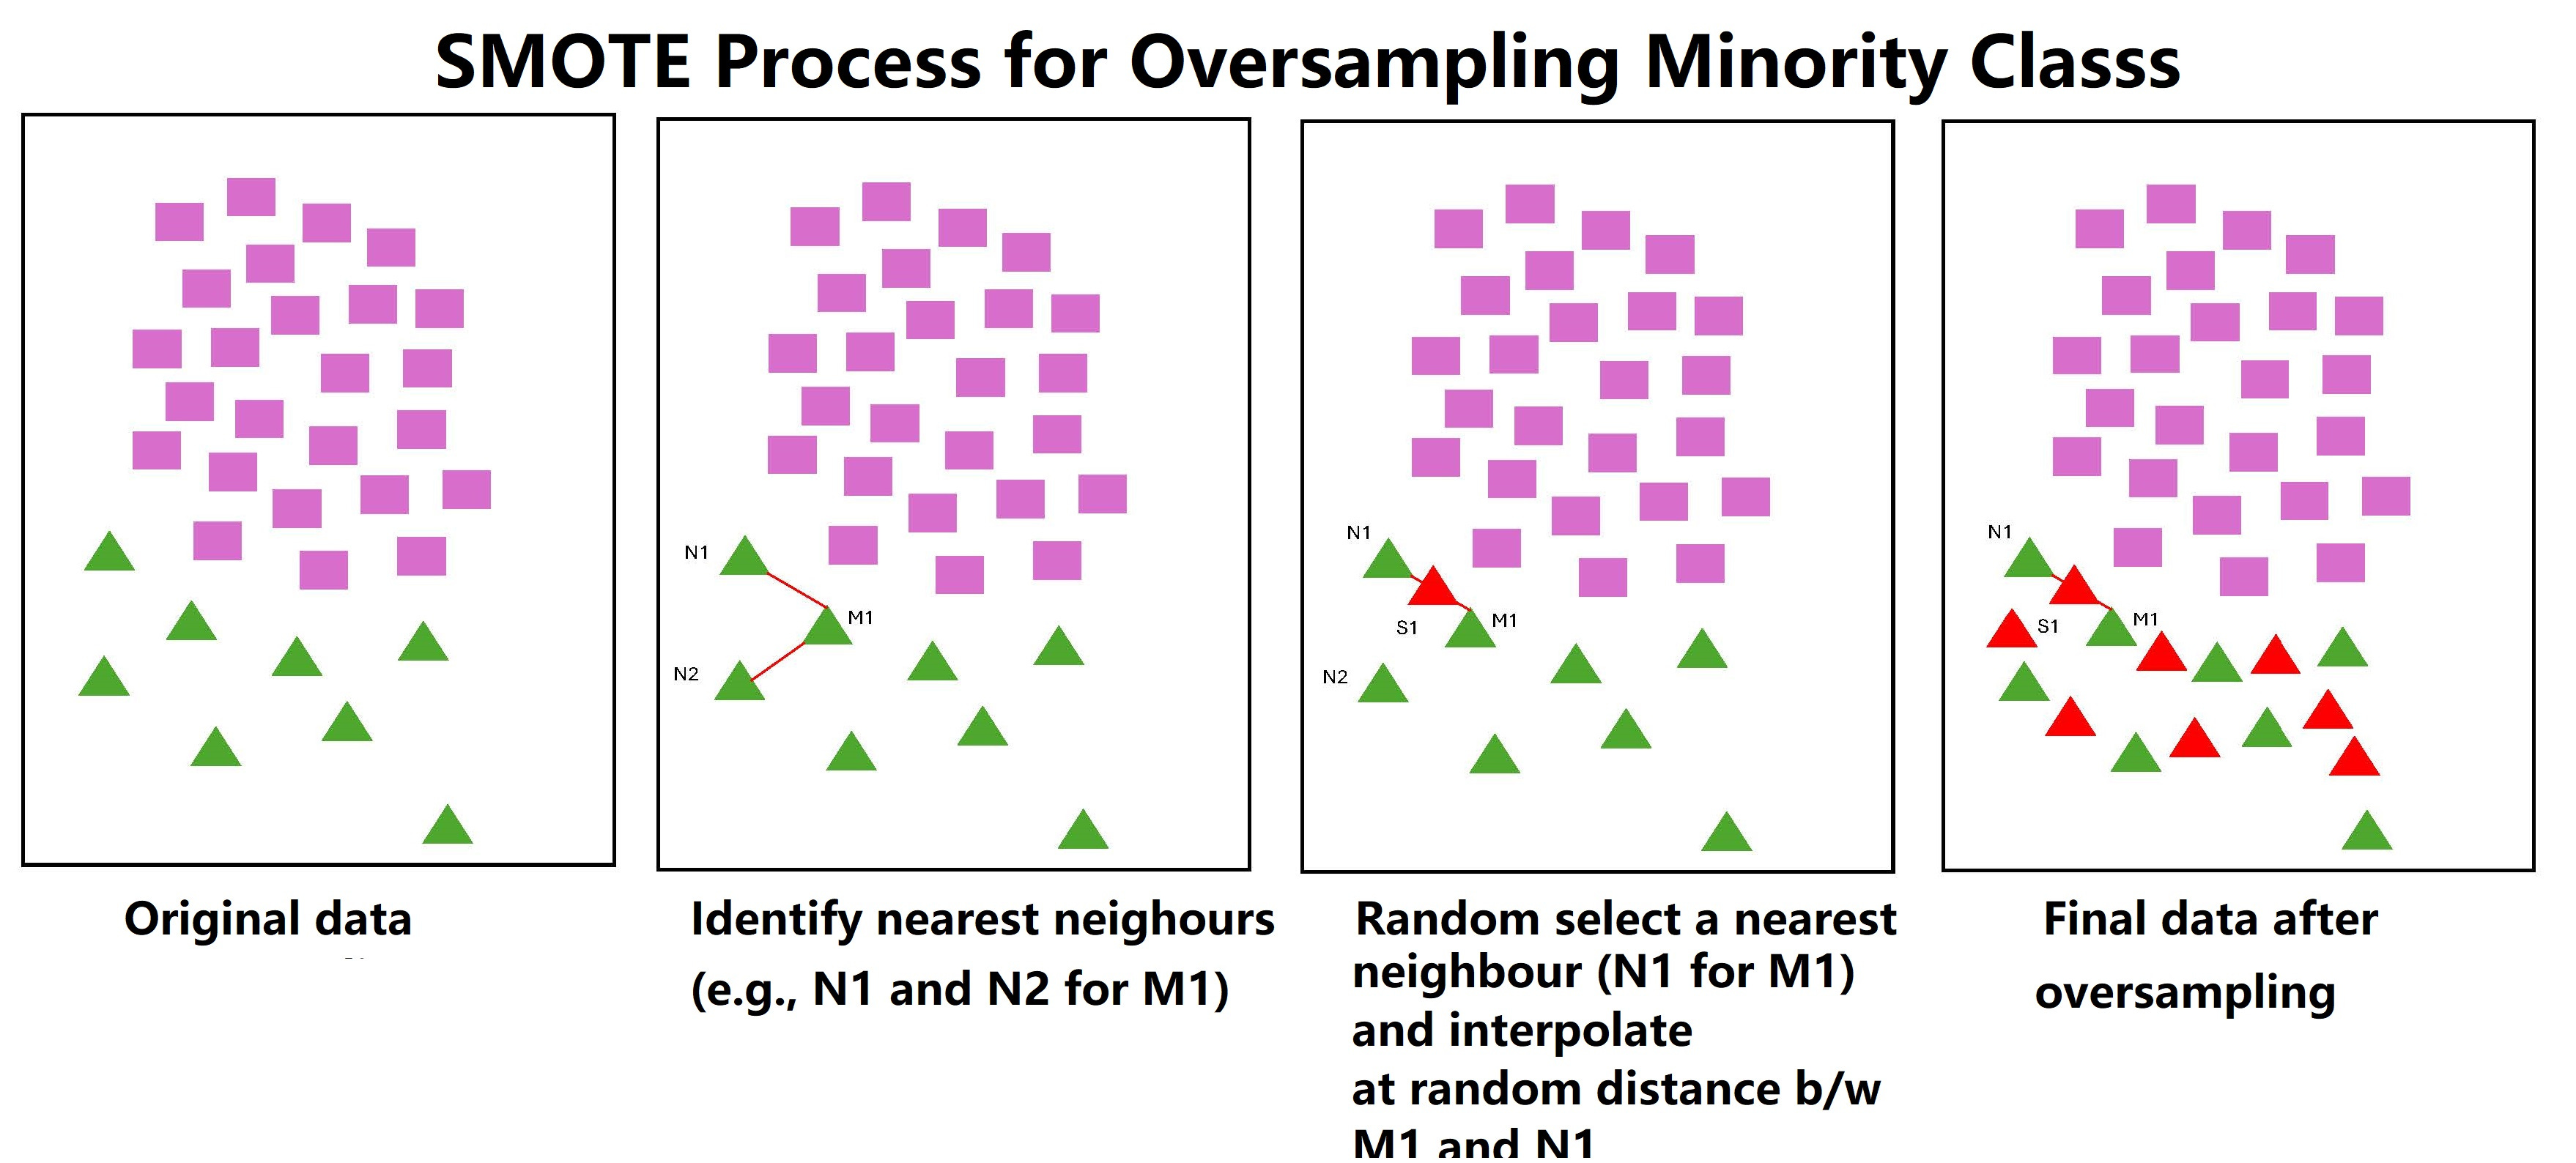
\includegraphics[height=0.5\textheight]{figures/img_p120_41.jpg}\par
  \raggedright
  \textbf{Nivel de algoritmo}:
  \begin{itemize}
    \item \textbf{Class weights}: penalizar más los errores en la minoría
    \item \textbf{Balanced loss}: pérdida ponderada por clase
    \item \textbf{Focal loss} (conceptual): concentrar el aprendizaje en los casos difíciles
  \end{itemize}
\end{frame}

% ============================================================ p122-123
\imageframe{figures/img_p123_42.png}

% ============================================================ p124
\begin{frame}{\texttt{class\_weight}: balanced loss}
  \begin{center}
    En lugar de cambiar los datos, se cambia cuánto pesa equivocarse en cada clase.
  \end{center}
  {\[ \mathcal{L} = -\frac{1}{n}\sum_{i=1}^{n} w_{y_i}\Big[y_i \log \hat{p}_i + (1 - y_i)\log(1 - \hat{p}_i)\Big] \qquad w_k = \frac{n}{K\, n_k} \]}
  \small
  \begin{itemize}
    \item $n$: observaciones; $K$: clases; $n_k$: observaciones de la clase $k$.
    \item \texttt{class\_weight="balanced"} implementa exactamente estos pesos.
    \item En árboles, los pesos modifican las proporciones $p_k$ usadas en Gini y Entropy.
  \end{itemize}
\end{frame}

% ============================================================ p125
\begin{frame}{\texttt{class\_weight}: qué gana y qué arriesga}
  \begin{columns}[T]
    \begin{column}{0.46\textwidth}
      \colhead{Puede ayudar a}
      \begin{itemize}
        \item aumentar atención sobre la clase rara;
        \item reducir falsos negativos;
        \item mantener todos los datos originales;
        \item crear una primera intervención simple.
      \end{itemize}
    \end{column}
    \begin{column}{0.46\textwidth}
      \begin{alertblock}{Cuidado}
        No garantiza mejor decisión. Puede mejorar recall y empeorar precision, por eso debe evaluarse con threshold y métrica correcta. Además distorsiona $\hat{p}$: recalibrar antes de usar probabilidades.
      \end{alertblock}
    \end{column}
  \end{columns}
\end{frame}

% ============================================================ B1 (nuevo)
\begin{frame}{Focal loss (conceptual)}
  \begin{columns}[c]
    \begin{column}{0.5\textwidth}
      \[ \mathcal{L}_{FL} = -\alpha_t\,(1 - \hat{p}_t)^{\gamma}\,\log \hat{p}_t \]
      \small $\hat{p}_t = \hat{p}$ si $y = 1$; $\hat{p}_t = 1 - \hat{p}$ si $y = 0$.
      \begin{itemize}
        \item $(1 - \hat{p}_t)^\gamma$ reduce el peso de los ejemplos fáciles (la mayoría de negativos obvios);
        \item $\gamma = 0$ recupera la cross-entropy ponderada;
        \item $\alpha_t$ balancea las clases;
        \item en boosting se usa como pérdida personalizada.
      \end{itemize}
      {\tiny Lin et al. (2017), \emph{Focal Loss for Dense Object Detection}.}
    \end{column}
    \begin{column}{0.46\textwidth}
      \centering
      \begin{tikzpicture}
        \begin{axis}[width=6cm,height=5cm,xmin=0,xmax=1,ymin=0,ymax=4,
          xlabel={\scriptsize $\hat{p}_t$},ylabel={\scriptsize pérdida},
          tick label style={font=\tiny},legend style={font=\tiny,draw=none},
          domain=0.02:1,samples=80]
          \addplot[mlgray,thick] {-ln(x)}; \addlegendentry{$\gamma=0$}
          \addplot[mlteal,thick] {-(1-x)*ln(x)}; \addlegendentry{$\gamma=1$}
          \addplot[mlgold,thick] {-(1-x)^2*ln(x)}; \addlegendentry{$\gamma=2$}
          \addplot[mlred,thick] {-(1-x)^5*ln(x)}; \addlegendentry{$\gamma=5$}
        \end{axis}
      \end{tikzpicture}
    \end{column}
  \end{columns}
\end{frame}

% ============================================================ p126
\begin{frame}{Under/oversampling: cambiar lo que el modelo ve}
  \begin{columns}[T]
    \begin{column}{0.46\textwidth}
      \colhead{Undersampling}
      \begin{itemize}
        \item reduce casos de la clase mayoritaria;
        \item acelera entrenamiento;
        \item puede perder información útil;
        \item depende mucho de cómo se selecciona.
      \end{itemize}
    \end{column}
    \begin{column}{0.46\textwidth}
      \colhead{Oversampling}
      \begin{itemize}
        \item aumenta casos de clase minoritaria;
        \item puede mejorar señal positiva;
        \item puede inducir overfitting;
        \item exige validación cuidadosa.
      \end{itemize}
    \end{column}
  \end{columns}
  \vspace{8pt}
  \begin{center}
    Cambiar la distribución de entrenamiento exige proteger la validación.
  \end{center}
\end{frame}

% ============================================================ p127
\begin{frame}{SMOTE no es magia}
  \begin{center}
    \large SMOTE crea ejemplos sintéticos de la clase minoritaria interpolando entre observaciones cercanas.\\[2pt]
    \footnotesize Variantes: \textbf{Borderline-SMOTE} (solo cerca de la frontera) y \textbf{ADASYN} (más sintéticos donde la clase es más difícil).
  \end{center}
  \begin{columns}[T]
    \begin{column}{0.46\textwidth}
      \colhead{Puede ser útil cuando}
      \begin{itemize}
        \item la clase positiva tiene pocos ejemplos;
        \item hay señal local aprovechable;
        \item se usa dentro del pipeline correcto;
        \item se valida sin contaminar el test.
      \end{itemize}
    \end{column}
    \begin{column}{0.46\textwidth}
      \begin{rulebox}[Riesgo metodológico]
        Si se aplica antes del split o fuera de la validación cruzada, puede introducir leakage y producir una comparación demasiado optimista.
      \end{rulebox}
    \end{column}
  \end{columns}
\end{frame}

% ============================================================ p128
\begin{frame}{Flujo incorrecto: rebalancing antes de dividir}
  \begin{center}
    \large Datos completos $\rightarrow$ SMOTE / oversampling $\rightarrow$ split $\rightarrow$ score optimista
  \end{center}
  \vspace{6pt}
  \begin{alertblock}{{\large Por qué falla}}
    \large La validación deja de representar el mundo real y puede recibir información derivada de observaciones que debían quedar fuera del entrenamiento.
  \end{alertblock}
\end{frame}

% ============================================================ p129
\begin{frame}[fragile]{Flujo defendible: rebalancing dentro de validación}
  \begin{center}
    Split / CV $\rightarrow$ rebalancing solo en train $\rightarrow$ validación en distribución natural
  \end{center}
\begin{lstlisting}[basicstyle=\ttfamily\scriptsize,columns=fullflexible,keepspaces=true]
from imblearn.pipeline import Pipeline
from imblearn.over_sampling import SMOTE

pipe = Pipeline([("smote", SMOTE(random_state=42)),
                 ("tree", DecisionTreeClassifier(max_depth=4))])
cross_val_score(pipe, X, y, cv=StratifiedKFold(5, shuffle=True, random_state=42),
                scoring="average_precision")
\end{lstlisting}
  \begin{alertblock}{Importante}
    Rebalancear solo en train, nunca en validación ni en test. La intervención es parte del pipeline evaluado.
  \end{alertblock}
\end{frame}

% ============================================================ B2 (nuevo)
\begin{frame}{Comparar estrategias de balanceo}
  \centering\scriptsize
  \begin{tabularx}{\textwidth}{@{}L{0.2\textwidth} c >{\raggedright\arraybackslash}X >{\raggedright\arraybackslash}X >{\raggedright\arraybackslash}X@{}}
    \toprule
    \hrow \textbf{Estrategia} & Nivel & Qué cambia & Efecto típico & Riesgo \\
    \midrule
    Random undersampling & datos & elimina mayoritarios & $\uparrow$ recall, $\downarrow$ precision & pierde información \\
    Random oversampling & datos & duplica minoritarios & $\uparrow$ recall & overfitting a duplicados \\
    SMOTE & datos & interpola minoritarios & $\uparrow$ recall & ruido; leakage fuera del fold \\
    Borderline-SMOTE & datos & interpola cerca de la frontera & $\uparrow$ recall en zona difícil & amplifica ruido de frontera \\
    ADASYN & datos & más sintéticos donde es difícil & $\uparrow$ recall & sensible a outliers \\
    Class weights / balanced loss & modelo & pondera la pérdida & $\uparrow$ recall & puede $\downarrow$ precision \\
    Focal loss & modelo & enfoca en casos difíciles & $\uparrow$ en difíciles & hiperparámetro $\gamma$ extra \\
    \bottomrule
  \end{tabularx}
  \vspace{6pt}

  \raggedright\small Todas alteran $\hat{p}$: recalibrar o elegir $\tau$ por validación.
\end{frame}

% ============================================================ p130
\begin{frame}{Discusión: ¿qué probaría primero?}
  \begin{taskbox}[\large Caso: primera intervención contra desbalance]
    \large Su baseline probabilístico detecta pocos fraudes. Debe proponer una primera estrategia para mejorar la lectura de la clase positiva sin destruir la validez del experimento.
  \end{taskbox}
  \vspace{2pt}
  \small
  \begin{columns}[T]
    \begin{column}{0.46\textwidth}
      \colhead{Elija y justifique}
      \begin{itemize}
        \item \texttt{class\_weight};
        \item undersampling;
        \item oversampling;
        \item SMOTE;
        \item focal loss (conceptual).
      \end{itemize}
    \end{column}
    \begin{column}{0.46\textwidth}
      \colhead{Debe declarar}
      \begin{itemize}
        \item métrica principal;
        \item esquema de CV;
        \item threshold a revisar;
        \item riesgo metodológico.
      \end{itemize}
    \end{column}
  \end{columns}
\end{frame}

% ============================================================ CVH0 (nuevo)
\section{Validación cruzada para HPO}
\sectionframe{Validación cruzada para\\optimización de hiperparámetros}

% ============================================================ CVH1
\begin{frame}[fragile]{La CV es la función objetivo de cada trial}
  \small Un \emph{trial} de Optuna propone hiperparámetros; la CV devuelve el número que el optimizador intenta maximizar.
\begin{lstlisting}[basicstyle=\ttfamily\scriptsize,columns=fullflexible,keepspaces=true,xleftmargin=12pt]
import optuna
from lightgbm import LGBMClassifier
skf = StratifiedKFold(5, shuffle=True, random_state=42)   # mismos folds en todos los trials

def objective(trial):
    params = {"learning_rate": trial.suggest_float("learning_rate", 1e-3, 0.3, log=True),
              "num_leaves": trial.suggest_int("num_leaves", 15, 255, log=True),
              "min_child_samples": trial.suggest_int("min_child_samples", 10, 200)}
    model = LGBMClassifier(n_estimators=500, **params)
    return cross_val_score(model, X_train, y_train, cv=skf,
                           scoring="average_precision").mean()

study = optuna.create_study(direction="maximize")
study.optimize(objective, n_trials=50)
\end{lstlisting}
  \begin{itemize}
    \item solo \texttt{X\_train}: el test no participa en ningún trial;
    \item el objeto \texttt{skf} fijo hace comparables todos los trials.
  \end{itemize}
\end{frame}

% ============================================================ CVH2
\begin{frame}{Elegir el tipo de fold según los datos}
  \centering\footnotesize
  \begin{tabular}{@{}L{0.3\textwidth} L{0.27\textwidth} L{0.33\textwidth}@{}}
    \toprule
    \hrow \textbf{Situación} & \textbf{Fold} & \textbf{Por qué} \\
    \midrule
    clases desbalanceadas & \texttt{StratifiedKFold} & cada fold conserva la prevalencia de positivos \\
    varias filas por cliente o tarjeta & \texttt{StratifiedGroupKFold} & un mismo grupo no aparece en train y validación \\
    datos con cronología & \texttt{TimeSeriesSplit} (con \texttt{gap}) & se entrena con el pasado y se valida con el futuro \\
    datos muy grandes o trials caros & holdout estratificado o 3 folds & menos costo por trial \\
    \bottomrule
  \end{tabular}
  \raggedright
  \begin{keybox}[Criterio]
    \small El fold debe imitar cómo llegarán los datos nuevos en producción. Si se elige mal, Optuna optimiza con precisión un score que no se va a repetir.
  \end{keybox}
\end{frame}

% ============================================================ CVH3
\begin{frame}{Por qué la CV debe definirse antes de la búsqueda bayesiana}
  \centering
  \begin{tikzpicture}[node distance=0.35cm,
      st/.style={fill=mlcream,minimum height=0.9cm,align=center,font=\scriptsize,text width=2.05cm},
      arr/.style={-{Stealth[length=2mm]},thick,eafitblue}]
    \node[st,fill=eafitsky] (a) {\textbf{1.} CV y métrica\\fijas};
    \node[st,right=of a] (b) {\textbf{2.} objetivo\\$f(\theta)$ = CV-score};
    \node[st,right=of b] (c) {\textbf{3.} optimizador\\bayesiano};
    \node[st,right=of c] (d) {\textbf{4.} mejor $\theta$,\\reentrenar en train};
    \node[st,right=of d,fill=mlredbg] (e) {\textbf{5.} una sola\\evaluación en test};
    \foreach \u/\v in {a/b,b/c,c/d,d/e} \draw[arr] (\u) -- (\v);
  \end{tikzpicture}
  \par\vspace{6pt}
  \raggedright\small
  \begin{itemize}
    \item el optimizador solo ve el número que devuelve la CV: \textbf{si la CV tiene leakage, lo optimiza con mucha eficiencia};
    \item cambiar folds o métrica a mitad del estudio vuelve incomparables los trials anteriores: el sustituto aprende de datos inconsistentes;
    \item una CV ruidosa (pocos positivos por fold) hace que el sustituto persiga ruido: estratificar o repetir la CV;
    \item muchos trials sobre la misma CV también sobreajustan a ella: por eso el test queda aparte.
  \end{itemize}
\end{frame}

% ============================================================ BO0 (nuevo)
\section{Optimización bayesiana}
\sectionframe{Optimización bayesiana con Optuna}

% ============================================================ BO1
\begin{frame}{La idea: construir un modelo del score}
  \begin{columns}[c]
    \begin{column}{0.46\textwidth}
      \centering
      \begin{tikzpicture}[st/.style={fill=mlcream,minimum width=2.5cm,minimum height=0.75cm,align=center,font=\scriptsize},
          arr/.style={-{Stealth[length=2mm]},thick,eafitblue}]
        \node[st] (p) at (0,1.5) {proponer $\theta$};
        \node[st,fill=eafitsky] (e) at (2,0) {evaluar CV-score($\theta$)};
        \node[st] (u) at (0,-1.5) {actualizar sustituto};
        \node[st] (a) at (-2,0) {maximizar adquisición};
        \draw[arr] (p) to[bend left=20] (e);
        \draw[arr] (e) to[bend left=20] (u);
        \draw[arr] (u) to[bend left=20] (a);
        \draw[arr] (a) to[bend left=20] (p);
      \end{tikzpicture}
    \end{column}
    \begin{column}{0.5\textwidth}
      \small
      \begin{itemize}
        \item evaluar la CV es caro; evaluar el \textbf{sustituto} es casi gratis;
        \item el sustituto estima el score (y su incertidumbre) en configuraciones no probadas;
        \item la \textbf{función de adquisición} decide dónde vale la pena gastar la siguiente evaluación;
        \item cada trial mejora el sustituto: la búsqueda se concentra en zonas buenas.
      \end{itemize}
    \end{column}
  \end{columns}
\end{frame}

% ============================================================ BO2
\begin{frame}{Modelos sustitutos: procesos gaussianos y TPE}
  \centering\footnotesize
  \begin{tabular}{@{}l L{0.37\textwidth} L{0.37\textwidth}@{}}
    \toprule
    \hrow & \textbf{Proceso gaussiano (GP)} & \textbf{TPE (Optuna por defecto)} \\
    \midrule
    \textbf{Qué modela} & $p(\text{score} \mid \theta)$: media $\mu(\theta)$ e incertidumbre $\sigma(\theta)$ & $p(\theta \mid \text{bueno}) = \ell(\theta)$ y $p(\theta \mid \text{malo}) = g(\theta)$ \\
    \textbf{Cómo elige} & maximiza EI o UCB sobre $\mu$ y $\sigma$ & separa los trials por un cuantil del score y elige $\theta$ que maximiza $\ell(\theta)/g(\theta)$ \\
    \textbf{Espacios} & continuos, pocas dimensiones & mixtos: enteros, categóricos, condicionales \\
    \textbf{Costo} & crece como $n^3$ con los trials & crece suave; escala a muchos trials \\
    \bottomrule
  \end{tabular}
  \raggedright
  \begin{keybox}[Lectura de TPE]
    \small ``Busca valores que aparecen seguido entre los mejores trials y poco entre los peores.''
  \end{keybox}
\end{frame}

% ============================================================ BO3
\begin{frame}{Funciones de adquisición: EI y UCB}
  \begin{columns}[T]
    \begin{column}{0.5\textwidth}
      \colhead{Expected Improvement (EI)}
      \[ \text{EI}(\theta) = \mathbb{E}\big[\max(f(\theta) - f^{*},\, 0)\big] \]
      \small ¿Cuánto espero superar al mejor score actual $f^{*}$? Premia $\mu$ alta y también $\sigma$ alta.
    \end{column}
    \begin{column}{0.46\textwidth}
      \colhead{Upper Confidence Bound (UCB)}
      \[ \text{UCB}(\theta) = \mu(\theta) + \kappa\,\sigma(\theta) \]
      \small Optimista frente a la incertidumbre. $\kappa$ grande explora más; $\kappa$ pequeño explota más.
    \end{column}
  \end{columns}
  \vspace{8pt}
  \begin{goldbox}[Ambas responden la misma pregunta]
    \small ¿Dónde es más probable encontrar algo mejor que lo que ya tengo, teniendo en cuenta lo que no sé?
  \end{goldbox}
\end{frame}

% ============================================================ BO4
\begin{frame}{Exploración frente a explotación}
  \begin{columns}[c]
    \begin{column}{0.56\textwidth}
      \centering
      \begin{tikzpicture}
        \begin{axis}[width=7.4cm,height=4.6cm,xmin=0,xmax=1,ymin=0.1,ymax=1.2,
          xlabel={\scriptsize hiperparámetro $\theta$},ylabel={\scriptsize CV-score},
          tick label style={font=\tiny},label style={font=\scriptsize},
          legend style={font=\tiny,draw=none,at={(0.5,-0.3)},anchor=north},legend columns=3,
          legend cell align=left,domain=0:1,samples=120]
          \addplot[name path=up,draw=none,forget plot] {0.5+0.22*sin(deg(5*x+0.3)) + 2*(0.02+0.12*(1-exp(-((x-0.1)^2)/0.006))*(1-exp(-((x-0.32)^2)/0.006))*(1-exp(-((x-0.45)^2)/0.006)))};
          \addplot[name path=lo,draw=none,forget plot] {0.5+0.22*sin(deg(5*x+0.3)) - 2*(0.02+0.12*(1-exp(-((x-0.1)^2)/0.006))*(1-exp(-((x-0.32)^2)/0.006))*(1-exp(-((x-0.45)^2)/0.006)))};
          \addplot[eafitsky,opacity=0.8] fill between[of=up and lo];
          \addlegendentry{incertidumbre $\mu \pm 2\sigma$}
          \addplot[eafitneon,thick] {0.5+0.22*sin(deg(5*x+0.3))};
          \addlegendentry{sustituto $\mu(\theta)$}
          \addplot[only marks,mark=*,mark size=1.8pt,mltext,samples at={0.1,0.32,0.45}] {0.5+0.22*sin(deg(5*x+0.3))};
          \addlegendentry{trials evaluados}
          \draw[-{Stealth[length=2mm]},mlteal,thick] (axis cs:0.3,1.02) -- (axis cs:0.3,0.8);
          \node[font=\tiny,text=mlteal] at (axis cs:0.3,1.09) {explotar};
          \draw[-{Stealth[length=2mm]},mlred,thick] (axis cs:0.85,1.12) -- (axis cs:0.85,0.86);
          \node[font=\tiny,text=mlred,anchor=east] at (axis cs:0.84,1.12) {explorar};
        \end{axis}
      \end{tikzpicture}
    \end{column}
    \begin{column}{0.42\textwidth}
      \small
      \begin{itemize}
        \item \textbf{explotar}: probar cerca del mejor trial, donde $\mu$ es alta y $\sigma$ baja;
        \item \textbf{explorar}: probar donde no hay trials y $\sigma$ es grande: ahí puede haber algo mejor;
        \item solo explotar se queda en un óptimo local; solo explorar es random search;
        \item Optuna empieza con trials aleatorios (\texttt{n\_startup\_trials}) antes de confiar en TPE.
      \end{itemize}
    \end{column}
  \end{columns}
\end{frame}

% ============================================================ BO5
\begin{frame}[fragile]{Early stopping dentro de cada trial}
\begin{lstlisting}[basicstyle=\ttfamily\scriptsize,columns=fullflexible,keepspaces=true,xleftmargin=12pt]
import lightgbm as lgb
def objective(trial):
    params = {"learning_rate": trial.suggest_float("learning_rate", 1e-3, 0.3, log=True),
              "num_leaves": trial.suggest_int("num_leaves", 15, 255, log=True),
              "subsample": trial.suggest_float("subsample", 0.5, 1.0), "subsample_freq": 1,
              "colsample_bytree": trial.suggest_float("colsample_bytree", 0.5, 1.0),
              "reg_lambda": trial.suggest_float("reg_lambda", 1e-3, 10, log=True)}
    scores = []
    for step, (tr, va) in enumerate(skf.split(X_train, y_train)):
        model = LGBMClassifier(n_estimators=2000, **params)   # alto: lo corta early stopping
        model.fit(X_train.iloc[tr], y_train.iloc[tr],
                  eval_set=[(X_train.iloc[va], y_train.iloc[va])],
                  callbacks=[lgb.early_stopping(100, verbose=False)])
        p = model.predict_proba(X_train.iloc[va])[:, 1]
        scores.append(average_precision_score(y_train.iloc[va], p))
    return np.mean(scores)
\end{lstlisting}
  \footnotesize\textbf{Early stopping} para de agregar árboles cuando la pérdida de validación deja de mejorar: elige \texttt{n\_estimators} dentro del trial. Usa el fold de validación, así que el score queda algo optimista: la evaluación final sigue siendo en test.
\end{frame}

% ============================================================ BO6
\begin{frame}[fragile]{Pruning: cortar trials que no prometen}
  \begin{columns}[T]
    \begin{column}{0.52\textwidth}
\begin{lstlisting}[basicstyle=\ttfamily\scriptsize,columns=fullflexible,keepspaces=true,numbers=none]
    # dentro del bucle de folds:
    trial.report(np.mean(scores), step)
    if trial.should_prune():
        raise optuna.TrialPruned()

study = optuna.create_study(
    direction="maximize",
    sampler=optuna.samplers.TPESampler(seed=42),
    pruner=optuna.pruners.MedianPruner(
        n_startup_trials=5))
study.optimize(objective, n_trials=100)
\end{lstlisting}
      \footnotesize \texttt{MedianPruner}: corta el trial si su score parcial queda bajo la mediana de los trials anteriores en el mismo paso.
    \end{column}
    \begin{column}{0.44\textwidth}
      \centering
      \begin{tikzpicture}
        \begin{axis}[width=5.6cm,height=4.4cm,xmin=0.8,xmax=5.2,ymin=0.2,ymax=0.8,
          xlabel={\scriptsize fold (paso)},ylabel={\scriptsize score parcial},
          tick label style={font=\tiny},label style={font=\scriptsize},xtick={1,...,5}]
          \addplot[mlgray,thick] coordinates {(1,0.55) (2,0.57) (3,0.58) (4,0.58) (5,0.59)};
          \addplot[mlgray,thick] coordinates {(1,0.5) (2,0.53) (3,0.52) (4,0.54) (5,0.55)};
          \addplot[eafitneon,very thick] coordinates {(1,0.6) (2,0.63) (3,0.64) (4,0.66) (5,0.67)};
          \addplot[mlred,thick,mark=x,mark size=3pt] coordinates {(1,0.36) (2,0.35)};
          \node[font=\tiny,text=mlred,anchor=west] at (axis cs:2.1,0.33) {podado en el paso 2};
          \node[font=\tiny,text=eafitneon,anchor=south] at (axis cs:3.2,0.66) {sigue};
        \end{axis}
      \end{tikzpicture}
      \par\footnotesize Early stopping corta \textbf{árboles} dentro de un modelo; pruning corta \textbf{trials} completos.
    \end{column}
  \end{columns}
\end{frame}

% ============================================================ BO7
\begin{frame}{Buenas prácticas con Optuna}
  \begin{columns}[T]
    \begin{column}{0.48\textwidth}
      \colhead{Antes y durante}
      \footnotesize
      \begin{itemize}
        \item fijar CV, métrica y semillas antes del primer trial;
        \item escala log para \texttt{learning\_rate}, \texttt{num\_leaves} y penalizaciones;
        \item presupuesto por número de trials o por tiempo (\texttt{timeout});
        \item guardar el estudio (\texttt{storage}) para poder retomarlo.
      \end{itemize}
    \end{column}
    \begin{column}{0.48\textwidth}
      \colhead{Después}
      \footnotesize
      \begin{itemize}
        \item revisar \texttt{plot\_optimization\_history} y \texttt{plot\_param\_importances};
        \item si el mejor valor está en el borde del rango, ampliarlo;
        \item reentrenar con \texttt{study.best\_params} en todo el train;
        \item elegir el threshold y calibrar en validación; evaluar una sola vez en test.
      \end{itemize}
    \end{column}
  \end{columns}
  \vspace{6pt}
  \begin{keybox}[En una frase]
    \small La búsqueda bayesiana gasta mejor el presupuesto, pero solo es tan buena como la CV que optimiza.
  \end{keybox}
\end{frame}

% ============================================================ H1 (nuevo)
\begin{frame}{Hands-on de la parte 2}
  \small
  \begin{enumerate}
    \item \textbf{SMOTE frente a \texttt{class\_weight}} dentro de la CV: mismo pipeline, mismos folds; comparar PR-AUC y calibración.
    \item \textbf{Optuna + LightGBM}: 50 trials con CV estratificada dentro del objetivo, early stopping y \texttt{MedianPruner}; comparar con el random search de la parte 1 al mismo presupuesto.
  \end{enumerate}
  \vspace{6pt}
  \begin{toolbox}[Notebook]
    \href{https://github.com/anvasquezre/EAFIT_AA_2026-02/blob/main/notebooks/02_ml_boosting_fraude.ipynb}{\textcolor{eafitneon}{\underline{\texttt{02\_ml\_boosting\_fraude.ipynb}}}} (local con \texttt{uv} o en Colab)
  \end{toolbox}
\end{frame}

% ============================================================ p131-132
\section{Cierre}
\sectionframe{Cierre}
\imageframe{figures/img_p132_43.png}

% ============================================================ glosario 2a
\begin{frame}{Glosario mínimo: árboles, boosting y optimización bayesiana}
  \small
  \begin{itemize}
    \item \textbf{CART / \texttt{ccp\_alpha}}: árbol binario por impureza / poda por costo-complejidad.
    \item \textbf{Bias--variance}: rigidez frente a sensibilidad al dataset observado.
    \item \textbf{Gradient boosting}: suma de árboles que ajustan el gradiente de la pérdida.
    \item \textbf{Por niveles / por hojas}: \texttt{max\_depth} (XGBoost) / \texttt{num\_leaves} (LightGBM).
    \item \textbf{Early stopping}: dejar de agregar árboles cuando la validación no mejora.
    \item \textbf{Sustituto (GP, TPE)}: modelo barato del CV-score según los hiperparámetros.
    \item \textbf{EI / UCB}: funciones de adquisición que equilibran explorar y explotar.
    \item \textbf{Pruning (Optuna)}: cortar trials cuyo score parcial queda bajo la mediana.
  \end{itemize}
\end{frame}

\begin{frame}{Glosario mínimo: ensembles y balanceo}
  \small
  \begin{itemize}
    \item \textbf{Ensemble / voting}: combinar predicciones de varios modelos.
    \item \textbf{Bagging / Random Forest}: agregación sobre muestras bootstrap; reduce variance.
    \item \textbf{Boosting}: aprendizaje secuencial que corrige errores; reduce bias.
    \item \textbf{Under / oversampling}: reducir la mayoría / aumentar la minoría.
    \item \textbf{SMOTE, Borderline-SMOTE, ADASYN}: generación sintética de minoritarios.
    \item \textbf{Balanced loss}: pérdida ponderada por clase (\texttt{class\_weight}).
    \item \textbf{Focal loss}: pérdida que reduce el peso de los ejemplos fáciles.
  \end{itemize}
\end{frame}

% ============================================================ preguntas 2
\begin{frame}{Preguntas que ya debe poder responder}
  \small
  \begin{enumerate}
    \item ¿Por qué combinar modelos reduce el error y qué requisito exige?
    \item ¿Bagging reduce bias o variance? ¿Y boosting?
    \item ¿Qué riesgo aparece si aplica SMOTE antes del split?
    \item ¿Qué diferencia hay entre SMOTE y Borderline-SMOTE?
    \item ¿Qué hace \texttt{class\_weight="balanced"} sobre la pérdida?
    \item ¿Qué hace el factor $(1 - \hat{p}_t)^\gamma$ de la focal loss?
    \item ¿Por qué hay que recalibrar después de rebalancear?
  \end{enumerate}
\end{frame}

% ============================================================ preguntas 2b
\begin{frame}{Preguntas que ya debe poder responder (II)}
  \small
  \begin{enumerate}\setcounter{enumi}{7}
    \item ¿Por qué un árbol profundo puede sobreajustar y cómo se poda?
    \item ¿Qué diferencia hay entre crecimiento por niveles y por hojas?
    \item ¿Qué palancas de regularización tiene LightGBM y qué efecto tiene cada una?
    \item ¿Por qué la CV debe definirse antes de la búsqueda bayesiana?
    \item ¿Qué hace la función de adquisición y qué significa explorar frente a explotar?
    \item ¿En qué se diferencian early stopping y pruning de Optuna?
  \end{enumerate}
\end{frame}

% ============================================================ p136
\begin{frame}{La frase técnica que debe sobrevivir}
  \large
  \begin{center}
    Un modelo no merece confianza porque su score se vea alto.\\[8pt]
    Merece confianza cuando el problema fue bien formulado, el baseline fue serio, la métrica fue correcta, la validación cruzada fue defendible y sin leakage, las probabilidades están calibradas y el threshold fue razonado.
  \end{center}
\end{frame}

% ============================================================ p137
\begin{frame}{Estándar del curso}
  \begin{center}
    \large En Aprendizaje Automático, no basta con entrenar modelos:\\[8pt]
    hay que defender decisiones de Machine Learning.
  \end{center}
  \vspace{6pt}
  \begin{keybox}[Transición]
    \small La próxima sesión profundiza en la teoría de XGBoost, LightGBM, CatBoost y otros modelos de boosting, sobre la misma CV y la misma búsqueda con Optuna.
  \end{keybox}
\end{frame}

% ============================================================ p138
\imageframe{figures/img_p138_44.png}

% ============================================================ p139
\begin{frame}[plain]
  \begin{tikzpicture}[remember picture,overlay]
    \node[anchor=north west,inner sep=0pt] at ([xshift=309pt,yshift=-45pt]current page.north west)
      {
\includegraphics[width=117pt]{figures/img_p139_45.png}};
    \node[anchor=north west,inner sep=0pt] at ([xshift=177pt,yshift=-191pt]current page.north west)
      {
\includegraphics[width=96pt]{figures/img_p139_46.png}};
    \node[anchor=center,align=center] at ([xshift=158pt,yshift=-90pt]current page.north west)
      {{\color{mltitle}\LARGE\bfseries Gracias por su atención}\\[6pt]
       {\color{mltitle}\normalsize ¿Preguntas, comentarios o discusión?}};
    \node[anchor=north,align=center,font=\footnotesize] at ([xshift=227pt,yshift=-143pt]current page.north west)
      {\textbf{Aprendizaje Automático}\\
       SI7009 · Universidad EAFIT};
  \end{tikzpicture}
\end{frame}

\end{document}
